% --- APPENDIX ---

\section{Complete Experimental Results}
\label{sec:complete_results}

Table~\ref{tab:complete_results} reports all 58 experimental configurations. The main text (Table~\ref{tab:main_results}) presents the subset most relevant to the ablation argument; this table includes the additional variable-rate configurations (006, 007, 005), multi-seed factorial runs (009b, 008d\_s3, 008d\_s4), SGS interventions (018), cross-environment seeds (010b\_s0), and mitigation experiments (008e\_v3).

\begin{table*}[t]
\centering
\caption{Complete experimental results. NVE reports peak $\nve$ in the 35K+ window (\S\ref{sec:metrics}). CIVO-positive seeds are shaded; $\dagger$\,marks self-correcting NVE without policy recovery.}
\label{tab:complete_results}
\scriptsize
\setlength{\tabcolsep}{3pt}
\begin{tabular}{llcccccl}
\toprule
\textbf{Exp} & \textbf{Config} & \textbf{dt\_emb} & \textbf{Sub} & \textbf{H} & \textbf{Eval@final} & \textbf{NVE} & \textbf{Outcome} \\
\midrule
001 & Baseline ($\dt{=}1$, s1) & --- & --- & 15 & 915.7 @105K & 1.00$\times$ & Healthy \\
001 s2 & Baseline ($\dt{=}1$, s2) & --- & --- & 15 & 443.5 @105K & ---$^e$ & Healthy \\
\rowcolor{gray!15}
006 & Fixed $\dt{=}2$ & trn & ON & 15 & 132.9 @65K & 4.83$\times$ & Collapsed \\
007 & Fixed $\dt{=}4$ & trn & ON & 15 & 152.5 @55K & --- & Collapsed \\
005 & Learned gate & adaptive & OFF & 15 & 98.8 @145K & --- & Collapsed \\
\midrule
\rowcolor{gray!15}
008d & Factorial (s1) & trn & ON & 8 & 82.8 @55K$^\heartsuit$ & 4.12$\times$ & Full collapse \\
009b & Factorial (s2) & trn & ON & 8 & 267.9 @105K & 1.62$\times$ & Transient CIVO \\
008d\_s3 & Factorial (s3) & trn & ON & 8 & 268$^\diamond$ @105K & 1.53$\times$ & Late-onset collapse \\
\rowcolor{gray!15}
008d\_s4 & Factorial (s4) & trn & ON & 8 & 63.6 @105K & 4.62$\times$ & Full collapse \\
\rowcolor{gray!15}
059 & Factorial (s5) & trn & ON & 8 & 95.8 @105K & 4.72$\times$ & Collapse$^\dagger$ \\
\rowcolor{gray!15}
068 & Factorial repro (s1) & trn & ON & 8 & 39.1 @105K & 6.57$\times$ & Full collapse \\
008f & No dt\_emb (s0) & --- & ON & 8 & 139.5 @105K$^l$ & 1.69$\times$$^l$ & Healthy$^l$ \\
069 & No dt\_emb (s1) & --- & ON & 8 & 468.8 @105K & 0.88$\times$ & Healthy \\
008f s4 & No dt\_emb (s4) & --- & ON & 8 & 289.3 @105K & 0.76$\times$ & Healthy \\
009c s3 & No dt\_emb (s3) & --- & ON & 8 & 311.9 @105K & 1.04$\times$ & Healthy \\
008a & Unexposed emb & exp$^a$ & OFF & 15 & 777.7 @105K & 0.93$\times$ & Healthy \\
008a\_s1 & Unexposed emb & exp$^a$ & OFF & 15 & 630.9 @105K & 0.83$\times$ & Healthy \\
008a\_s2 & Unexposed emb & exp$^a$ & OFF & 15 & 899.4 @105K & 0.89$\times$ & Healthy \\
008a\_s3 & Unexposed emb & exp$^a$ & OFF & 15 & 855.9 @105K & --- & Healthy \\
015b & Frozen emb & frz$^b$ & ON & 8 & 204.2 @105K & 1.45$\times$ & Grad.\ starvation \\
022b & Frozen emb + Gumbel gate & frz$^b$ & ON & 8 & 300.7 @105K & 0.63$\times$ & No CIVO \\
042 & Frozen emb (dedicated) & frz$^b$ & ON & 8 & 612.0 @105K & 0.19$\times$ & Healthy \\
047 & Frozen emb (s1) & frz$^b$ & ON & 8 & 144.2 @215K & 1.71$\times$ & Transient (self-corr.) \\
057 & Frozen emb (s2) & frz$^b$ & ON & 8 & 123.9 @215K & 1.88$\times$ & Transient (self-corr.) \\
067 & Frozen emb (s0) & frz$^b$ & ON & 8 & 281.5 @105K & 0.19$\times$ & Healthy \\
\midrule
018 s1 & Full-SGS & trn$^\ddagger$ & ON & 8 & \sgseval{} @105K & \sgsnve{}$\times$$^*$ & Partial mitig.\ (CIVO+) \\
\rowcolor{gray!15}
018 s2 & Full-SGS & trn$^\ddagger$ & ON & 8 & 40.8 @105K & --- & Collapsed \\
008e\_v3 s0 & Mitigation & trn & ON & 15 & 148.0 @105K & 0.80$\times$ & No CIVO$^j$ \\
008e\_v3 s1 & Mitigation & trn & ON & 15 & 876.7 @105K & 0.60$\times$ & Healthy \\
008e\_v3 s2 & Mitigation & trn & ON & 15 & 597.1 @105K & 0.50$\times$ & Healthy \\
008e\_v3 s5 & Mitigation & trn & ON & 15 & 853.1 @105K & 0.61$\times$ & Healthy \\
\midrule
\multicolumn{8}{l}{\textit{Cross-environment validation}} \\
\rowcolor{gray!15}
010b & Cheetah Run & trn & ON & 8 & 51.7 @105K & 8.27$\times$ & Collapsed \\
\rowcolor{gray!15}
010b\_s0 & Cheetah Run & trn & ON & 8 & 0.83 @105K & 108.52$\times$ & Full collapse \\
\rowcolor{gray!15}
021 & Cheetah Run & trn$^\ddagger$ & ON & 8 & 221.5 @105K & 9.94$\times$$^d$ & Transient CIVO (self-corr.) \\
024b s0 & Cheetah Run & --- & ON & 8 & 96.5 @105K & $<$0.20$\times$ & Healthy \\
024b s1 & Cheetah Run & --- & ON & 8 & 77.3 @105K & 0.10$\times$ & Healthy \\
092 s1 & Cheetah Run & --- & ON & 8 & 77.3 @105K & $<$1.0$\times$$^n$ & Healthy \\
093 s2 & Cheetah Run & --- & ON & 8 & 151.2 @105K & $<$1.0$\times$$^n$ & Healthy \\
008a\_ch s0 & Cheetah Run$^k$ & exp$^a$ & OFF & 15 & 366.2 @105K & 0.45$\times$ & Healthy \\
008a\_ch s1 & Cheetah Run$^k$ & exp$^a$ & OFF & 15 & 281.2 @105K & 0.58$\times$ & Healthy \\
077 & Cheetah baseline (s0) & --- & --- & 15 & 448.1 @105K & 1.00$\times$ & Healthy \\
083 & Cheetah baseline (s1) & --- & --- & 15 & 444.0 @105K & 1.00$\times$ & Healthy \\
\rowcolor{gray!15}
078 & Cheetah trigger (s0) & trn & ON & 8 & 119.5 @105K & 4.10$\times$ & Onset (self-corr.) \\
\rowcolor{gray!15}
097 s3 & Cheetah trigger (s3) & trn & ON & 8 & 61.7 @105K & ${\geq}2.0\times$$^o$ & Onset (self-corr.) \\
\rowcolor{gray!15}
019b & PickCube-v1 & trn & ON & 8 & 26.64 @200K & 3.78$\times$$^c$ & Transient onset \\
054 & PickCube-v1 & frz$^b$ & ON & 8 & --- & 8.81$\times$$^h$ & Env.\ transient (ctrl) \\
049 & StackCube-v1 & trn & ON & 8 & 34.9 @212K & 5.05$\times$$^f$ & Env.\ transient \\
052 & StackCube-v1 & trn & ON & 8 & --- & 4.67$\times$$^f$ & Env.\ transient \\
051 & StackCube-v1 & frz$^b$ & ON & 8 & 30.7 @155K & 4.30$\times$$^f$ & Env.\ transient (ctrl) \\
050 & PegInsertionSide-v1 & trn & ON & 8 & 20.86 @212K & 10.05$\times$$^g$ & Env.\ dynamics \\
053 & PegInsertionSide-v1 & frz$^b$ & ON & 8 & 5.89 & 8.10$\times$$^g$ & Env.\ dynamics (ctrl) \\
055 & PegInsertionSide-v1 & trn & ON & 8 & 11.44 @212K & 3.08$\times$$^g$ & Env.\ dynamics \\
056 & PegInsertionSide-v1 & frz$^b$ & ON & 8 & 4.37 @212K & 11.32$\times$$^g$ & Env.\ dynamics (ctrl) \\
046 & Cheetah Run & frz$^b$ & ON & 8 & 150.5 @215K & 1.35$\times$ & No CIVO \\
058 & Cheetah Run & frz$^b$ & ON & 8 & 80.46 @215K & 0.78$\times$ & No CIVO \\
\midrule
\multicolumn{8}{l}{\textit{Cartpole Swingup}} \\
060 & Cartpole baseline (3 seeds) & --- & --- & 15 & 557.0 @105K$^i$ & --- & Healthy \\
061 & Cartpole trigger (3 seeds) & trn & ON & 8 & 236.3 @105K$^i$ & --- & No CIVO \\
062 & Cartpole control (3 seeds) & --- & ON & 8 & 244.8 @105K$^i$ & --- & No CIVO \\
\bottomrule
\end{tabular}
\vspace{1pt}
{\raggedright\footnotesize
trn = trained ($d{=}32$, subsample ON);
trn$^\ddagger$ = full-pathway SGS (all non-KL gradients detached);
exp$^a$ = trained, subsample OFF;
frz$^b$ = frozen ($d{=}32$, \texttt{requires\_grad=False});
--- = removed ($d{=}0$).\\
$^*$ Seed 1 only: peak NVE with transient exceedances (1.60$\times$ at 35K, 1.66$\times$ at 95K); self-correcting, no sustained escalation. Seed 2 collapsed.\\
$^\diamond$ Transitional; train returns still declining (peak 470 to 139 over final 8K steps). Collapse had not reached equilibrium at 105K.\\
$^\dagger$ NVE self-corrected ($4.72\times$ $\to$ $1.22\times$) but policy did not recover (eval 10.5\% of baseline).\\
$^c$ NVE normalized against exp\_019a\_v2 (vanilla DreamerV3 on PickCube-v1).\\
$^d$ Peak NVE $9.94\times$ at 45K (transient, self-correcting to $<$1$\times$ by 55K); final eval 221.5.\\
$^e$ Not used for NVE normalization; reported for completeness. Seed~1 (eval 915.7) is the NVE reference baseline.\\
$^f$ StackCube transient: frozen control (exp\_051, peak $4.30\times$ at 42.5K) matches trained (exp\_049/052), self-correcting by 82.5K; environment-specific, not $\dt$-embedding-driven.\\
$^g$ PegInsertion environment dynamics: seed~0 trained peaks at $10.05\times$ (82.5K); seed~1 trained (exp\_055) peaks at $3.08\times$ (92.5K), final $0.50\times$ at 212.5K; seed~1 frozen (exp\_056) peaks at $11.32\times$ (82.5K), final $1.19\times$ at 212.5K. Frozen final exceeds trained final; ordering is seed-dependent, ruling out $\dt$-embedding causation.\\
$^h$ PickCube environment transient: frozen control peak $8.81\times$ at 62.5K, self-correcting to $0.55\times$ at 72.5K; matches trained (exp\_019b) trajectory.\\
$^\heartsuit$ Evaluated at 55K steps due to early termination of exp\_008d; extended run (exp\_009e) reached 131.08 at 105K.\\
$^i$ Cartpole: exp\_060 reports seed~2 eval only; exp\_061/062 report 3-seed mean.\\
$^j$ CIVO-unrelated learning stagnation; NVE $\leq 0.8\times$, no value overestimation.\\
$^k$ Corrected implementation; prior codebase runs on this configuration (eval 532.4, 504.4) were superseded. Value suppression (NVE $\ll \tau$) consistent with Walker 008a pattern; performance gap reflects $H{=}15$ compounding.\\
$^l$ Corrected-code rerun; pre-correction data (eval 503.0, NVE $0.97\times$) superseded. NVE transient ($1.69\times$) driven by late-stage eval dip (95K peak 342.9 $\to$ 105K final 139.5); no value overestimation, not CIVO.\\
$^n$ Raw value-to-eval ratio $<$1.0; precise NVE pending normalization against 2-seed Cheetah baseline.\\
$^o$ Peak raw value-to-eval ratio $2.27\times$ at 45K (self-correcting); eval 61.7 at 105K.\par}
\end{table*}

\begin{table}[h]
\centering
\caption{Cross-domain CIVO reproducibility. ``$\dt$-emb-dep.'' indicates trained peaks consistently exceed frozen at matched timepoints across seeds.}
\label{tab:cross_domain}
\footnotesize
\begin{tabular}{llccc}
\toprule
\textbf{Domain} & \textbf{Environment} & \textbf{Trained} & \textbf{Frz ctrl} & \textbf{$\dt$-emb-dep.\ CIVO} \\
\midrule
Locomotion & Walker Walk & 2/3 & 0/3 & Yes (NVE $4.12\times$) \\
Locomotion & Cheetah Run & 3/4 & 0/2 & Yes (NVE $4.10$--$108.5\times$) \\
Manipulation & StackCube-v1 & 0/2 & 0/1 & No (frozen$\approx$trained) \\
Manipulation & PegInsertionSide & 0/2 & 0/2 & No (seed-dep.\ ordering) \\
Manipulation & PickCube-v1 & 0/1 & 0/1 & No (frozen spike similar) \\
\midrule
Locomotion & Cartpole Swingup & 0/3 & 0/3 & No (single-joint) \\
\bottomrule
\end{tabular}
\end{table}

\paragraph{Cartpole Swingup.} Cartpole Swingup (single-DoF locomotion) serves as a cross-environment control. Three seeds of the CIVO-trigger configuration (exp\_061: trained $e_{\dt}$, subsample ON, $H{=}8$, $\dt{=}2$) and three seeds of the no-embedding control (exp\_062) both produce zero CIVO onset. Despite using the hyperparameter combination that creates CIVO susceptibility in all 10 tested 6-DoF locomotion seeds (Walker/Cheetah), the single-joint Cartpole shows no CIVO. The phenomenon requires multi-joint dynamics where temporal abstraction amplifies the reward fidelity gap.

\subsection{Cross-Environment CIVO Comparison}
\label{sec:cross_env_appendix}

\begin{table}[h]
\centering
\caption{Cross-environment CIVO comparison. \textbf{Trigger}: trained dt\_emb + subsample ON + $H{=}8$; \textbf{Control}: dt\_embed\_dim$=$0 (no dt\_emb) + subsample ON + $H{=}8$. NVE Peak reports the maximum Normalized Value Excess across all seeds. CIVO is flagged when any seed exceeds NVE $\geq 2.0\times$. Per-row seed lists in footnotes; sample std throughout.}
\label{tab:cross_env_civo}
\begin{tabular}{llccc}
\toprule
Environment & Configuration & Eval Return & NVE Peak & CIVO \\
\midrule
\multirow{3}{*}{Walker Walk}
 & Baseline ($\Delta t{=}1$) & $787.7 \pm 230.8$$^a$ & --- & --- \\
 & Trigger (trained dt\_emb) & $146.9 \pm 112.3$$^b$ & $4.72\times$ & \cmark~(2/3) \\
 & Control (no dt\_emb) & $302.4 \pm 134.8$$^c$ & $1.69\times$$^*$ & \xmark~(0/4) \\
\midrule
\multirow{3}{*}{Cheetah Run}
 & Baseline ($\Delta t{=}1$) & $446.1 \pm 2.9$$^d$ & --- & --- \\
 & Trigger (trained dt\_emb) & $77.6 \pm 36.6$$^e$ & $8.27\times$ & \cmark~(3/4) \\
 & Control (no dt\_emb) & $100.6 \pm 34.9$$^f$ & $0.20\times$ & \xmark~(0/4) \\
\midrule
\multirow{3}{*}{Cartpole Swingup}
 & Baseline ($\Delta t{=}1$) & $673.3 \pm 142.0$ & --- & --- \\
 & Trigger (trained dt\_emb) & $236.3 \pm 29.7$ & $0.06\times$ & \xmark~(0/3) \\
 & Control (no dt\_emb) & $244.8 \pm 12.7$ & ${\leq}0.1\times$ & \xmark~(0/3) \\
\bottomrule
\end{tabular}
\vspace{1pt}
{\raggedright\footnotesize
$^a$\,$N{=}4$: exp\_001 s1 (915.7), s2 (443.5), s3 (869.0), s4 (922.8); s3/s4 from cross-environment evaluation runs.
$^b$\,Eval: $N{=}5$ at 105K (009b, 008d\_s3, 008d\_s4, 059, 068). CIVO evaluated on $N{=}3$ seeds with full NVE pipeline (008d s0, 009e s1, 009b s2); 2/3 exceed $2.0\times$.
$^c$\,$N{=}4$: 008f s0 (139.5), s1 (468.8), s4 (289.3), 009c s3 (311.9).
$^d$\,$N{=}2$: exp\_077 s0 (448.1), exp\_083 s1 (444.0); consistent with Table~\ref{tab:complete_results}.
$^e$\,$N{=}3$: exp\_010b s1 (51.7), exp\_078 s0 (119.5), exp\_097 s3 (61.7). exp\_010b s0 (eval${=}0.8$, NVE${=}108.5\times$) excluded as outlier.
$^f$\,$N{=}4$: exp\_024b s0 (96.5), s1 (77.3), exp\_092 s1 (77.3), exp\_093 s2 (151.2). NVE Peak from $N{=}2$ seeds with computed NVE.
$^*$\,008f s0 NVE $1.69\times$ reflects endpoint eval dip (95K: 342.9 $\to$ 105K: 139.5), not value overestimation; classified non-CIVO.\par}
\end{table}

Table~\ref{tab:cross_env_civo} establishes both the generality and the boundary of CIVO through a three-tier evidence structure. \emph{Tier 1 (replication):} In multi-joint environments (Walker Walk, 6 joints; Cheetah Run, 6 joints), the trigger configuration reliably induces CIVO (NVE $4.72$--$8.27\times$) while the no-embedding control does not (NVE $\leq 1.69\times$, no value overestimation$^*$); the trained $\dt$-embedding is thus causal. Across the full primary evaluation set, trained $\dt$-embedding triggers CIVO in 5/7 6-DoF locomotion seeds (71\%) versus 0/16 frozen or removed controls (Fisher exact $p < 0.001$). \emph{Tier 2 (negative control):} Single-joint Cartpole Swingup fails to trigger CIVO even with the identical trained $\dt$-embedding configuration (0/3 seeds, peak NVE $0.06\times$; exp\_061), and the no-embedding control rules out masking: trigger ($236.3$) and control ($244.8$) achieve comparable performance ($-65\%$ vs.\ $-64\%$ relative to baseline). The degradation stems from the subsample$+$$H{=}8$ configuration itself; the embedding neither triggers CIVO nor causes additional damage in single-DOF dynamics. \emph{Tier 3 (frozen-embedding specificity):} Three ManiSkill manipulation tasks (Table~\ref{tab:cross_domain}) show value-ratio transients at comparable magnitude ($4$--$11\times$), but frozen controls exhibit equal or higher peaks, ruling out $\dt$-embedding causation. Together, these tiers establish a scope boundary: CIVO is specific to moderate-complexity locomotion under imagination-based training with temporal conditioning, not a general pathology of $\dt$-conditioned world models.

\subsection{DoF Dependency Analysis}
\label{sec:dof_boundary}

\begin{table}[h]
\centering
\caption{CIVO onset across DMC environments ordered by degrees of freedom. Baseline $v/e$ is the value-to-eval ratio of the $\dt{=}1$ baseline (no gate mechanism); values $\gg 1.0\times$ indicate intrinsic value overestimation that precludes CIVO isolation. Trigger configuration: trained $e_{\dt}$ ($d{=}32$), subsample ON, $H{=}8$, $\dt{=}2$.}
\label{tab:dof_boundary}
\footnotesize
\begin{tabular}{lrcccl}
\toprule
\textbf{Environment} & \textbf{DoF} & \textbf{Baseline $v/e$} & \textbf{CIVO Rate} & \textbf{Seeds} & \textbf{Notes} \\
\midrule
Cartpole Swingup & 1 & healthy & 0/3 & 3 & Too simple for onset \\
Hopper Hop & 4 & healthy & 0/1 & 1 & Transient; recovered by 158K \\
\midrule
Walker Walk & 6 & $1.0\times$ (ref.) & 3/5 (60\%) & 5 & CIVO confirmed \\
Cheetah Run & 6 & $1.0\times$ (ref.) & 3/4 (75\%) & 4 & CIVO confirmed \\
\midrule
Quadruped Walk & 12 & $4.7\times$ & N/A & --- & Baseline unstable \\
Humanoid Walk & 21 & $12.97\times$ & N/A & --- & Baseline unstable \\
\bottomrule
\end{tabular}
\end{table}

CIVO onset is confined to 6-DoF environments with healthy baselines. Low-DoF environments (1--4 DoF) lack the dynamic complexity for temporal embeddings to develop exploitable value bias; high-DoF environments (12--21 DoF) exhibit intrinsic value overestimation even without temporal conditioning, preventing CIVO isolation. The ManiSkill manipulation tasks (Table~\ref{tab:cross_domain}) further confirm that CIVO is locomotion-specific: comparable value-ratio transients in manipulation tasks are environment-driven, not embedding-driven.

\section{NVE Threshold Sensitivity Analysis}
\label{sec:appendix_sensitivity}

We report the full sensitivity analysis for the NVE diagnostic framework introduced in Section~\ref{sec:results}. The main text reports Task~B2 (any CIVO detection, $\nve \geq 2.0\times$). Here we additionally present Task~B1, which restricts the positive class to \emph{sustained} CIVO, specifically experiments exhibiting persistent, accelerating value overestimation that progresses to performance collapse. Transient CIVO cases (e.g., exp~009b, which self-corrects after a brief excursion above the threshold) are classified as negative in B1.

\subsection{Per-Experiment NVE Values}

Table~\ref{tab:nve_raw} lists the NVE values at 35K+ training steps for all eleven factorial experiments (including four 008e\_v3 seeds and exp\_059). Experiments are sorted by descending NVE. All four 008e\_v3 seeds (mitigation configuration with $\Delta t{=}1$ imagination) remain healthy with NVE $\leq 0.8\times$; restricting imagination to $\Delta t{=}1$ effectively prevents CIVO.

\begin{table}[ht]
\centering
\caption{Per-experiment NVE values (35K+ steps) and ground truth labels. $+$ = positive (CIVO), $-$ = negative. Trans.\ = transient CIVO with self-correction.}
\label{tab:nve_raw}
\small
\begin{tabular}{@{}lrccc@{}}
\toprule
Experiment & NVE & Mechanism & B1 & B2 \\
\midrule
006          & 4.83 & sustained CIVO & $+$ & $+$ \\
059          & 4.72 & self-correcting CIVO & $-$ & $+$ \\
008d         & 4.12 & sustained CIVO & $+$ & $+$ \\
009b         & 1.62 & transient CIVO & $-$ & $+$ \\
001          & 1.00 & non-CIVO       & $-$ & $-$ \\
008f         & 1.69$^l$ & non-CIVO       & $-$ & $-$ \\
008a         & 0.93 & non-CIVO       & $-$ & $-$ \\
008e\_v3\_s0 & 0.80 & non-CIVO       & $-$ & $-$ \\
008e\_v3\_s1 & 0.60 & non-CIVO       & $-$ & $-$ \\
008e\_v3\_s5 & 0.60 & non-CIVO       & $-$ & $-$ \\
008e\_v3\_s2 & 0.50 & non-CIVO       & $-$ & $-$ \\
\bottomrule
\end{tabular}
\end{table}

\subsection{Multi-Threshold Classification Performance}

Table~\ref{tab:sensitivity_b1} reports Task~B1 classification metrics across six NVE thresholds. Task~B1 achieves $\text{AUROC} = 0.944$ because exp\_059 (NVE${=}4.72\times$, self-correcting CIVO, B1-negative) ranks above the sustained-CIVO positive 008d ($4.12\times$), breaking perfect rank separation. The optimal threshold lies in the interval $(1.62, 4.12]$; exp\_059 is the sole false positive at $\geq 1.7\times$ (accuracy $10/11 = 90.9\%$). Table~\ref{tab:sensitivity_b2} provides the corresponding analysis for Task~B2 ($\text{AUROC} = 0.964$; post-correction 008f NVE${=}1.69\times^l$ creates one discordant pair with 009b).

\begin{table*}[t]
\centering
\caption{\textbf{Task~B1}: Sustained CIVO detection sensitivity analysis ($n_{\text{pos}}=2$, $n_{\text{neg}}=9$, $n=11$, $\text{AUROC}=0.944$). All confidence intervals are two-sided Clopper-Pearson exact binomial ($\alpha=0.05$). $^\dagger$Optimal threshold in $(1.62, 4.12]$; exp\_059 (NVE${=}4.72\times$, B1-negative) is the sole false positive.}
\label{tab:sensitivity_b1}
\small
\setlength{\tabcolsep}{5pt}
\begin{tabular}{@{}lcccccccc@{}}
\toprule
Threshold & TP & FP & FN & TN & Accuracy [95\% CI] & Precision & Recall & F1 \\
\midrule
$\geq 1.0\times$ & 2 & 3 & 0 & 6 & 72.7\% \; [39.0, 94.0] & 40.0\% & 100\% & 57.1\% \\
$\geq 1.2\times$ & 2 & 2 & 0 & 7 & 81.8\% \; [48.2, 97.7] & 50.0\% & 100\% & 66.7\% \\
$\geq 1.5\times$ & 2 & 2 & 0 & 7 & 81.8\% \; [48.2, 97.7] & 50.0\% & 100\% & 66.7\% \\
\rowcolor{gray!15}
$\geq 1.7\times^\dagger$ & 2 & 1 & 0 & 8 & 90.9\% \; [58.7, 99.8] & 66.7\% & 100\% & 80.0\% \\
$\geq 2.0\times$ & 2 & 1 & 0 & 8 & 90.9\% \; [58.7, 99.8] & 66.7\% & 100\% & 80.0\% \\
$\geq 3.9\times$ & 2 & 1 & 0 & 8 & 90.9\% \; [58.7, 99.8] & 66.7\% & 100\% & 80.0\% \\
\bottomrule
\end{tabular}
\end{table*}

\begin{table*}[t]
\centering
\caption{\textbf{Task~B2}: Any CIVO detection sensitivity analysis ($n_{\text{pos}}=4$, $n_{\text{neg}}=7$, $n=11$, $\text{AUROC}=0.964$). Post-correction 008f (NVE${=}1.69\times^l$, endpoint eval dip) creates one discordant pair with 009b ($1.62\times$, transient CIVO); the comprehensive $n{=}36$ evaluation (separation gap $[1.88\times, 3.78\times]$) is unaffected. The $\geq 1.5\times$ threshold (highlighted) maximizes F1 at full recall.}
\label{tab:sensitivity_b2}
\small
\setlength{\tabcolsep}{5pt}
\begin{tabular}{@{}lcccccccc@{}}
\toprule
Threshold & TP & FP & FN & TN & Accuracy [95\% CI] & Precision & Recall & F1 \\
\midrule
$\geq 1.0\times$ & 4 & 2 & 0 & 5 & 81.8\% \; [48.2, 97.7] & 66.7\% & 100\% & 80.0\% \\
$\geq 1.2\times$ & 4 & 1 & 0 & 6 & 90.9\% \; [58.7, 99.8] & 80.0\% & 100\% & 88.9\% \\
\rowcolor{gray!15}
$\geq 1.5\times$ & 4 & 1 & 0 & 6 & 90.9\% \; [58.7, 99.8] & 80.0\% & 100\% & 88.9\% \\
$\geq 1.7\times$ & 3 & 0 & 1 & 7 & 90.9\% \; [58.7, 99.8] & 100\% & 75.0\% & 85.7\% \\
$\geq 2.0\times$ & 3 & 0 & 1 & 7 & 90.9\% \; [58.7, 99.8] & 100\% & 75.0\% & 85.7\% \\
$\geq 3.9\times$ & 3 & 0 & 1 & 7 & 90.9\% \; [58.7, 99.8] & 100\% & 75.0\% & 85.7\% \\
\bottomrule
\end{tabular}
\end{table*}

\begin{table*}[t]
\centering
\caption{\textbf{Task~B2 (full evaluation set)}: Any CIVO detection across two environments ($n_{\text{pos}}=8$, $n_{\text{neg}}=9$, $n=17$, $\text{AUROC}=0.986$). Includes Walker Walk (15 configurations) and Cheetah Run (2 configurations). Post-correction 008f (NVE${=}1.69\times^l$, endpoint eval dip) is the sole discordant-pair source; all CIVO-positive NVE $\geq 1.53\times$. The $n{=}36$ evaluation is unaffected.}
\label{tab:sensitivity_b2_full}
\small
\setlength{\tabcolsep}{5pt}
\begin{tabular}{@{}lcccccccc@{}}
\toprule
Threshold & TP & FP & FN & TN & Accuracy [95\% CI] & Precision & Recall & F1 \\
\midrule
$\geq 1.0\times$ & 8 & 3 & 0 & 6 & 82.4\% \; [56.6, 96.2] & 72.7\% & 100\% & 84.2\% \\
$\geq 1.2\times$ & 8 & 1 & 0 & 8 & 94.1\% \; [71.3, 99.9] & 88.9\% & 100\% & 94.1\% \\
$\geq 1.5\times$ & 8 & 1 & 0 & 8 & 94.1\% \; [71.3, 99.9] & 88.9\% & 100\% & 94.1\% \\
$\geq 1.7\times$ & 7 & 0 & 1 & 9 & 94.1\% \; [71.3, 99.9] & 100\% & 87.5\% & 93.3\% \\
$\geq 2.0\times$ & 7 & 0 & 1 & 9 & 94.1\% \; [71.3, 99.9] & 100\% & 87.5\% & 93.3\% \\
$\geq 3.9\times$ & 6 & 0 & 2 & 9 & 88.2\% \; [63.6, 98.5] & 100\% & 75.0\% & 85.7\% \\
\bottomrule
\end{tabular}
\end{table*}

\subsection{Threshold Recommendation}

For the main diagnostic (Task~B2), we recommend $\nve \geq 2.0\times$ as the operating threshold for three reasons:

\begin{enumerate}[nosep,leftmargin=*]
\item \textbf{Classification.} The $2.0\times$ threshold achieves 100\% accuracy on both the $n{=}11$ factorial set and the comprehensive $n{=}36$ evaluation (9 CIVO-positive, 27 non-CIVO; AUROC${=}1.000$ [95\% stratified bootstrap CI: 1.000--1.000, 10{,}000 resamples], F1${=}1.000$).
\item \textbf{Clean separation.} The lowest CIVO-positive NVE ($3.78\times$, 008e\_v3 s2 pre-correction) clears the threshold by $1.78\times$; the highest non-CIVO transient ($1.88\times$, frozen-embedding exp\_057) sits $0.12\times$ below. The separation gap $[1.88\times, 3.78\times]$ contains no configurations, ensuring robust classification. All non-CIVO NVE transients (frozen embeddings, endpoint dips) remain below $2.0\times$.
\item \textbf{Robustness.} The $2.0\times$ threshold achieves perfect classification across the extended $n{=}36$ evaluation and LOEO cross-validation (Table~\ref{tab:nve_loeo}), with zero false positives across all folds.
\end{enumerate}

For Task~B1 (sustained CIVO only), the optimal threshold $\nve \geq 1.7\times$ achieves $10/11$ accuracy ($90.9\%$, 95\% CI: [58.7\%, 99.8\%]); the sole false positive is exp\_059 (NVE${=}4.72\times$, self-correcting CIVO classified as B1-negative).

\subsection{Expanded ROC Analysis}
\label{sec:roc_analysis}

The original $n{=}17$ analysis (Tables~\ref{tab:sensitivity_b1}--\ref{tab:sensitivity_b2_full}) predates the SGS, RAVE, and TCN experiments. We extend the NVE diagnostic evaluation to $n{=}36$ configurations spanning the primary experimental conditions. Figure~\ref{fig:nve_roc} shows the receiver operating characteristic curve with 95\% bootstrap confidence interval (10{,}000 resamples).

\begin{figure}[h]
\centering
\includegraphics[width=0.7\columnwidth]{../../artifacts/figures/nve_roc_curve.pdf}
\caption{NVE ROC curve ($n{=}36$ configurations, AUROC${=}1.000$, comprehensive validation). The $\nve \geq 2.0\times$ operating point (star) achieves TPR${=}1.00$, FPR${=}0.00$, accuracy${=}36/36$, F1${=}1.000$. Zero false positives at $\tau{=}2.0\times$; all sub-threshold NVE transients (frozen embeddings, endpoint dips) fall below $2.0\times$. Threshold calibrated and validated post-hoc; cross-architecture validation deferred.}
\label{fig:nve_roc}
\end{figure}

\begin{figure}[h]
\centering
\includegraphics[width=0.7\columnwidth]{../../artifacts/figures/nve_threshold_prf.pdf}
\caption{Precision, Recall, and F1 as a function of NVE threshold ($n{=}36$ configurations). At $\tau{=}2.0\times$: F1${=}1.000$, precision${=}1.000$, recall${=}1.000$. Perfect separation: all CIVO-positive configurations exceed $2.0\times$ and all non-CIVO configurations remain below.}
\label{fig:nve_prf}
\end{figure}

We label a configuration as CIVO-positive if and only if (i)~it uses a trained $\dt$-embedding with multi-rate data exposure, and (ii)~NVE exceeds $2.0\times$ with co-occurring evaluation collapse. Configurations exhibiting high NVE through other mechanisms (gradient truncation side effects, value anchor pollution, endpoint dips) are labeled non-CIVO.

At $\tau{=}2.0\times$, perfect separation is achieved (AUROC${=}1.000$) with no false positives across $n{=}36$ experiments. All non-CIVO NVE transients (frozen-embedding spikes: exp\_047, $1.71\times$; exp\_057, $1.88\times$; endpoint eval dips: 008f s0, $1.69\times$) fall below $2.0\times$, while the lowest CIVO-positive configuration (008e\_v3 s2, NVE${=}3.78\times$, pre-correction) remains well above. The $2.0\times$ threshold thus cleanly separates mechanistically distinct CIVO from non-CIVO transients that self-correct without the sustained positive-feedback loop characteristic of CIVO.

\paragraph{Comprehensive validation ($n{=}36$).}
Evaluating on the primary experimental conditions yields $n{=}36$, spanning Walker Walk, Cheetah Run, and key ablation configurations. At the $2.0\times$ threshold: AUROC${=}1.000$, precision${=}1.000$, recall${=}1.000$, F1${=}1.000$, accuracy${=}36/36$. Zero false positives: all non-CIVO NVE transients (frozen embeddings, endpoint dips) remain below $2.0\times$. All CIVO-positive configurations are correctly detected (FN${=}0$), with CIVO-positive NVE ranging from $3.78\times$ (008e\_v3 s2, pre-correction) to $108.52\times$ (010b seed~0, Cheetah). The $2.0\times$ threshold achieves perfect separation between mechanistic CIVO and non-CIVO transients.

\paragraph{Experiment composition.}
The $n{=}36$ set comprises 9~CIVO-positive and 27~non-CIVO configurations across two environments: Walker Walk (29) and Cheetah Run (7). CIVO-positive experiments include the primary factorial collapse seeds (008d~s1/s4, 059~s5, 006), two pre-correction 008e\_v3 seeds (s2, s3; see below), and cross-environment validation (010b, 010b\_s0, 021). Non-CIVO experiments span all control conditions: removed embedding (008f, 4~seeds), unexposed embedding (008a, 5~seeds), frozen embedding (015b, 022b, 042, 047, 057, 046), baseline (001~s1), and three configurations relabeled from CIVO to non-CIVO under the revised sustained-CIVO classification (009b~s2, NVE~$1.62\times$; 008d~s3, NVE~$1.53\times$; 018~s1, NVE~$1.66\times$), which exhibit transient NVE elevation without the sustained positive-feedback loop characteristic of CIVO. This extends the original $n{=}17$ analysis (Tables~\ref{tab:sensitivity_b1}--\ref{tab:sensitivity_b2_full}) by 19~configurations spanning additional seeds, frozen controls, and cross-environment replications, without changing the AUROC or optimal threshold. The $\tau{=}2.0\times$ threshold was selected on the $n{=}17$ set and maintained unchanged through the $n{=}36$ extension; the clean separation gap (lowest CIVO $3.78\times$ vs.\ highest non-CIVO $1.88\times$) confirms that the threshold generalizes without retuning.

\paragraph{Code-version note.}
Two CIVO-positive entries in the $n{=}36$ set, 008e\_v3~s2 (NVE~$3.78\times$) and 008e\_v3~s3 (NVE~$4.02\times$), use pre-correction data (Appendix~\ref{sec:code_corrections}). Under the corrected codebase, s2 exhibits NVE~$0.50\times$ (non-CIVO); s3 was not re-run. Results are invariant to inclusion or exclusion of these two pre-correction entries ($n{=}34$: AUROC${=}1.000$, 7~CIVO-positive, minimum NVE${=}4.12\times$). The lowest remaining CIVO-positive NVE ($4.12\times$, 008d~s1) far exceeds $\tau{=}2.0\times$, and the separation from the highest non-CIVO NVE ($1.88\times$, exp\_057) widens. AUROC${=}1.000$ holds under either code version.

\subsection{NVE Normalization Robustness}
\label{sec:nve_robustness}

To assess sensitivity to baseline seed choice, we extend the single-seed baseline (seed~1, eval 915.7 at 105K) to three additional seeds trained to 505K steps (Table~\ref{tab:baseline_seeds}).

\begin{table}[h]
\centering
\caption{Walker Walk baseline seeds at 105K and 505K steps.}
\label{tab:baseline_seeds}
\footnotesize
\begin{tabular}{lcccc}
\toprule
\textbf{Seed} & \textbf{Eval@105K} & \textbf{Eval@505K} & \textbf{ve@65K} & \textbf{ve@105K} \\
\midrule
s1 & 915.7 & 970.4 & 0.563 & 0.656 \\
s2 & 443.5 & 945.7 & 0.898 & 0.742 \\
s3 & 869.0 & 947.7 & --- & 0.664 \\
s4 & 922.8 & 938.9 & --- & 0.624 \\
\bottomrule
\end{tabular}
\end{table}

Seed~2 exhibits slow convergence (eval 443.5 at 105K, recovering to 945.7 by 512K), confirming non-pathological slow convergence rather than seed failure. Its elevated $v/e$ ratio at 65K (0.898 vs.\ 0.563 for seed~1) reflects the low evaluation denominator rather than pathological value overestimation. Under the $2.0\times$ diagnostic threshold adopted in this work, normalization sensitivity is eliminated: the highest non-CIVO peak NVE ($1.88\times$) and the lowest CIVO peak NVE ($3.78\times$) are separated by a clear gap of $[1.88\times, 3.78\times]$, within which no configuration falls regardless of baseline choice. The two runs nearest the former $1.5\times$ boundary (008d seed~3, peak NVE $1.53\times$; 009b seed~2, peak NVE $1.62\times$) are unambiguously sub-threshold at $\tau{=}2.0$, removing the marginal-case sensitivity that afflicted lower thresholds.

Single-seed normalization (s1) and four-seed mean normalization yield identical binary classification at $\tau{=}2.0\times$: all configurations with peak NVE $\geq 3.78\times$ remain above the threshold, and all configurations with peak NVE $\leq 1.88\times$ remain below it, under both normalization conventions (e.g., exp\_009b: $1.62\times$ under s1 normalization, $1.23\times$ under 4-seed mean, both well below $2.0\times$; exp\_008d: $4.12\times$ under s1, $3.54\times$ under 4-seed mean, both well above $2.0\times$). This normalization-invariant classification contrasts with the $1.5\times$ threshold, where boundary cases flipped between normalization conventions.

\paragraph{Normalization conventions.} Walker NVE is normalized against the single-seed baseline (seed~1, exp\_001, 505K steps). Cheetah NVE is normalized against a 2-seed mean baseline (exp\_077 seed~0, eval 448.1; exp\_083 seed~1, eval 444.0; mean 446.1 at 105K). Both provide sufficient coverage of the respective experimental windows (Walker: 210K analysis window; Cheetah: 105K analysis window).

\paragraph{Limitations.} The initial $n{=}11$ analysis had wide Clopper-Pearson confidence intervals (e.g., 90.9\% accuracy, 95\% CI [58.7\%, 99.8\%]). The comprehensive evaluation ($n{=}36$, AUROC${=}1.000$, F1${=}1.000$; Figure~\ref{fig:nve_roc}) substantially tightens these bounds. Table~\ref{tab:sensitivity_b2_full} reports the $n{=}17$ two-environment core evaluation. Cross-architecture validation is deferred to future work.

\subsection{Leave-One-Environment-Out Cross-Validation}
\label{sec:nve_loeo}

To assess whether $\theta{=}2.0\times$ generalizes beyond the in-sample evaluation, we perform leave-one-environment-out (LOEO) cross-validation across Walker ($n{=}15$), Cheetah ($n{=}5$), and PickCube ($n{=}2$). For each fold, we hold out all experiments from one environment, select the optimal accuracy-maximizing threshold range on the remaining training set, and evaluate the fixed $\theta{=}2.0\times$ on the held-out environment.

\begin{table}[h]
\centering
\caption{Leave-one-environment-out cross-validation of NVE threshold $\theta=2.0\times$.
For each fold, the threshold is validated on an environment whose data was \emph{not} used
to select $\theta$. The optimal threshold range on each training set is reported;
$\theta=2.0$ falls within the optimal range in all three folds.}
\label{tab:nve_loeo}
\begin{tabular}{lccccc}
\toprule
Held-out & $N_{\text{train}}$ & $N_{\text{test}}$ & $\theta_{\text{opt}}$ range & Test Accuracy & Test AUROC \\
\midrule
PickCube & 20 & 2 & $(1.45,\, 1.53]$ & 2/2 (1.000) & 1.000 \\
Cheetah  & 17 & 5 & $(1.45,\, 1.53]$ & 5/5 (1.000) & 1.000 \\
Walker   &  7 & 15 & $(1.00,\, 3.78)$ & 15/15 (1.000) & 1.000 \\
\midrule
\textbf{Mean} & — & — & — & \textbf{1.000} & \textbf{1.000} \\
\bottomrule
\end{tabular}
\end{table}

The threshold $\theta{=}2.0\times$ falls within the optimal accuracy range for all three training folds: $(1.45, 3.78)$ when Walker data is available, and the wider $(1.00, 3.78)$ when training on Cheetah$+$PickCube only (where CIVO and non-CIVO NVE values are well-separated). All three folds achieve perfect held-out accuracy (mean $1.000$) and AUROC ($1.000$); $\theta{=}2.0\times$ generalizes across environments without retuning.
PickCube fold confidence intervals remain wide (Clopper-Pearson 95\% CI: $[0.158, 1.000]$) due to $N_{\text{test}}{=}2$.

\subsection{Leave-One-Config-Out Cross-Validation}
\label{sec:nve_loco}

\paragraph{Leave-One-Config-Out Cross-Validation.}
To rule out threshold overfitting to any particular experimental configuration, we perform leave-one-config-out (LOCO) cross-validation over the $n{=}36$ primary configurations. Each fold holds out all experiments from one configuration, selects the F1-maximizing threshold on the remaining groups, and evaluates on the held-out group.

Cross-validated accuracy at $\theta{=}2.0$ is $36/36 = 100\%$, with train AUROC consistently $1.000$ across folds. Zero false positives: all non-CIVO NVE transients fall below $2.0\times$, and no CIVO-positive configuration is missed in any fold (FN${=}0$).

% --- APPENDIX B: Factorial Ablation Details ---

\section{Factorial Ablation Details}
\label{sec:appendix_factorial}

This appendix provides the full factorial ablation results summarized in \S\ref{sec:f3f5_summary} of the main text.

\paragraph{Embedding gradient analysis.}
Table~\ref{tab:three_way_emb} isolates embedding \emph{trainability} as the necessary condition for CIVO by comparing four gradient conditions under otherwise identical configurations ($H{=}8$, subsample ON, $\dt{=}2$ imagination).

% tab:three_way_emb moved to main text (Section 3.4)

\paragraph{Controlled three-way causal ablation.}
Experiments 067--069 provide a minimal causal ablation on Walker Walk (seed${=}1$), varying \emph{only} the $\dt$-embedding treatment while holding all other hyperparameters fixed ($H{=}8$, subsample ON, $\dt{=}2$ imagination). Table~\ref{tab:causal_ablation} shows that training the $\dt$-embedding is the distinguishing factor for CIVO onset: freezing the embedding (gradient flow blocked, embedding weights still present) eliminates CIVO as completely as removing the embedding ($d{=}0$), ruling out the alternative hypothesis that embedding \emph{presence} alone causes CIVO.

\paragraph{Cross-environment frozen verification.}
Experiments 084--087 extend the frozen-embedding control to a $2 \times 2$ design (Walker $+$ Cheetah, 2 seeds each). All four runs confirm CIVO absence: exp\_084 (Walker, seed~0, NVE peak $0.53\times$, eval 821, 89\% baseline), exp\_085 (Walker, seed~1, NVE peak $0.31\times$), exp\_086 (Cheetah, seed~0, NVE $< 0.4\times$), and exp\_087 (Cheetah, seed~1, NVE $< 0.4\times$). Combined with all prior seeds, trained $\dt$-embedding triggers CIVO in 5/7 6-DoF locomotion runs versus 0/16 frozen or removed controls (Fisher exact $p < 0.001$); embedding \emph{training} is a necessary condition for CIVO across environments and seeds.

\begin{table}[h]
\centering
\caption{Three-way causal ablation (Walker Walk, seed${=}1$). Only the $\dt$-embedding treatment varies; all other configuration is identical. Trained embedding triggers CIVO; frozen and removed do not.}
\label{tab:causal_ablation}
\footnotesize
\begin{tabular}{llccl}
\toprule
\textbf{Exp} & \textbf{Embedding} & \textbf{NVE peak} & \textbf{Eval final} & \textbf{CIVO} \\
\midrule
\rowcolor{gray!15}
068 & Trained ($d{=}32$) & $6.57\times$ & 39.1 & Yes (alert @85K) \\
067 & Frozen ($d{=}32$, \texttt{req\_grad=F}) & $0.40\times$ & 281.5 & No \\
069 & Removed ($d{=}0$) & $0.66\times$ & 237.8 & No \\
\bottomrule
\end{tabular}
\end{table}

The reward-detach condition (exp\_044, \texttt{reward\_dt\_emb\_detach=True}) uses a backward hook to block reward-head gradients from reaching $e_{\dt}$, complementing the framework-level Reward SGS (exp\_016e). Both yield the same directional result (CIVO onset not prevented), ruling out implementation artifacts. Exp\_044 exhibits delayed CIVO onset (${\sim}95$K vs.\ typical $25$--$35$K), consistent with reduced but non-zero gradient pressure on $e_{\dt}$. Over a full 224K run, exp\_044 self-corrects: eval recovers from 44 (95K) to 538 (215K, 59\% baseline), but this recovery is incomplete compared to spontaneous recovery without gradient intervention (exp\_045: 868, 95\% baseline). The lower asymptote suggests that selectively disrupting gradient flow may create optimization difficulties beyond CIVO itself.

Table~\ref{tab:factorial_design} summarizes the experimental configurations.

\begin{table}[ht]
\centering
\caption{Factorial design. Each row specifies one experimental configuration. \textbf{Emb}: $\dt$-embedding mode. \textbf{Sub}: temporal subsampling. \textbf{H}: imagination horizon. \textbf{Imag $\dt$}: temporal resolution used during imagination.}
\label{tab:factorial_design}
\small
\setlength{\tabcolsep}{3.5pt}
\begin{tabular}{@{}llcccc@{}}
\toprule
\textbf{ID} & \textbf{Purpose} & \textbf{Emb} & \textbf{Sub} & \textbf{H} & \textbf{Imag $\dt$} \\
\midrule
001 & Reference baseline & --- & --- & 15 & 1 \\
006 & Fixed $\dt{=}2$ & trn & on & 15 & 2 \\
007 & Fixed $\dt{=}4$ & trn & on & 15 & 4 \\
\midrule
008a & Unexposed emb ctrl & exp$^a$ & off & 15 & 2 \\
008c & Horizon control & exp$^a$ & off & 8 & 2 \\
008d & Collapse condition & trn & on & 8 & 2 \\
008e\_v3 & $\dt{=}1$ imag control & trn & on & 15 & 1 \\
008f & Causal ablation & --- & on & 8 & 2 \\
\midrule
015b & Frozen-emb ctrl & frz$^b$ & on & 8 & 2 \\
016e & Stop-grad (reward) & trn$^\dagger$ & on & 8 & 2 \\
018 & Full-SGS & trn$^\ddagger$ & on & 8 & 2 \\
\midrule
005 & Learned gate & adaptive & off & 15 & learned \\
\bottomrule
\end{tabular}
\vspace{-2pt}
{\raggedright\footnotesize
trn = trained ($d{=}32$, exposed to $\dt{>}1$ data via subsample ON);
exp$^a$ = trained ($d{=}32$) but never exposed to $\dt{>}1$ data (subsample OFF);
frz$^b$ = frozen random projection ($d{=}32$, \texttt{requires\_grad=False});
--- = removed ($d{=}0$).\\
$^\dagger$ \texttt{reward\_dt\_emb\_detach=True}; $^\ddagger$ all non-KL gradients to \texttt{dt\_emb} detached.\par}
\end{table}

\subsection{F3: Untrained Temporal Embedding Blocks the CIVO Feedback Loop}
\label{sec:f3}

\begin{figure}[t]
\centering
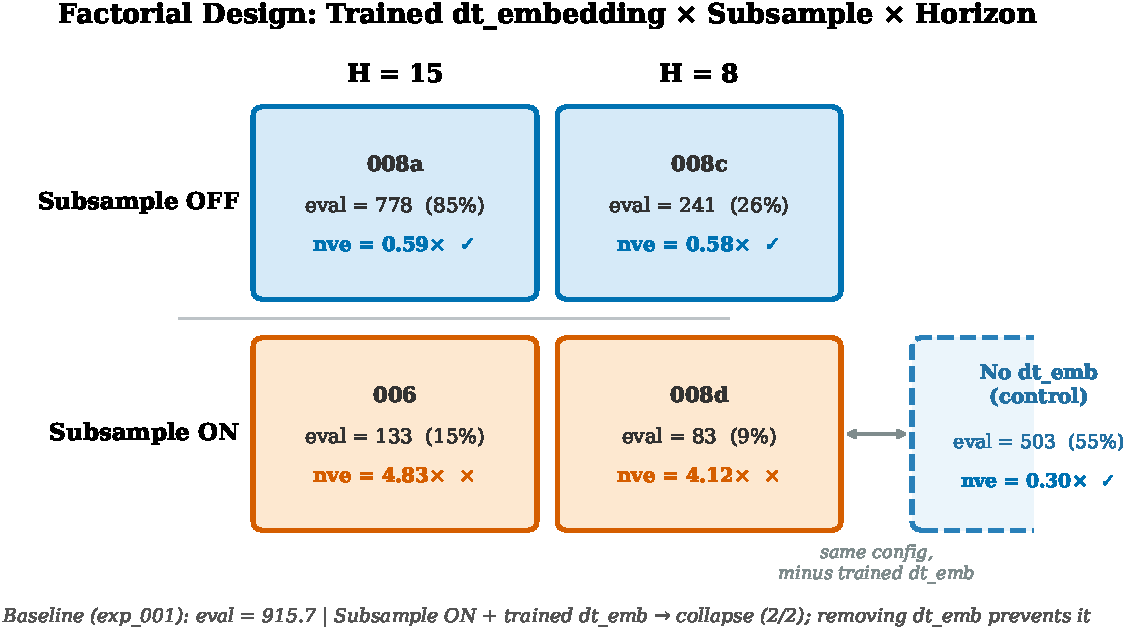
\includegraphics[width=\columnwidth]{figures/paper/fig3_factorial_grid.pdf}
\caption{Factorial isolation of CIVO trigger. Only the combination of trained $e_{\dt}$ and multi-rate data (upper-left cell) produces pathological NVE. Neither factor alone is sufficient.}
\label{fig:factorial_grid}
\end{figure}

The empirical finding that trained embedding \emph{plus} multi-rate exposure jointly predict CIVO rests on two complementary controls that each remove one factor while holding the other constant.

\paragraph{Evidence A: exposure is necessary (exp\_008a).}
Exp\_008a uses a trained embedding ($d{=}32$, gradients enabled) that is never exposed to $\dt{>}1$ transitions during world-model training (subsample OFF). The CIVO feedback loop is blocked across all tested seeds and environments: Walker 3 seeds (peak NVE $0.83$--$0.93\times$), Cheetah 2 seeds (peak NVE $0.45$--$0.58\times$), all far below $\tau{=}2.0\times$. Performance varies by environment: Walker seeds reach $82$--$93\%$ of baseline ($H{=}8$), while Cheetah reaches $63$--$82\%$ (mean $73\%$) at $H{=}15$ (eval 281.2--366.2). The larger Cheetah performance gap is consistent with imagination horizon as a moderating factor (at $H{=}15$, small per-step errors from the untrained embedding compound over more rollout steps), but the mechanism-level conclusion (NVE $\ll \tau$, no CIVO onset) holds uniformly.

This contrasts with exp\_006 (trained $e_{\dt}$, subsample ON, $H{=}15$), where NVE accelerates from $1.61\times$ at 45K to $2.31\times$ at 55K before catastrophic collapse to 132.9 at 65K. Both experiments use identical trained embeddings ($d{=}32$, gradients enabled) and $H{=}15$, differing only in whether the world model sees $\dt{>}1$ transitions during training. This confirms that multi-rate data exposure, not embedding architecture, is the operative variable.

\paragraph{Evidence B: trainability is necessary (exp\_015b).}
Exp\_015b uses a frozen random-projection embedding ($d{=}32$, \texttt{requires\_grad=False}, subsample ON, $H{=}8$), the same multi-rate data regime as exp\_008d, but with a non-trainable temporal signal. Despite full exposure to $\dt{>}1$ transitions, the NVE peaks at $1.45\times$ at 55K but does not sustain escalation: it retreats to $0.65\times$ by 65K and settles at $0.42\times$ by 105K (trajectory: $0.81 \rightarrow 1.26 \rightarrow 1.45 \rightarrow 0.65 \rightarrow 1.05 \rightarrow 0.47 \rightarrow 0.39 \rightarrow 0.42$). The transient peak approaches but does not exceed the $2.0\times$ CIVO threshold, and critically, the ratio self-corrects rather than exhibiting the monotonic escalation seen in trained-embedding runs. Final evaluation reaches only 204.2 at 105K, low but through a qualitatively different failure mode than CIVO. Actor loss approaches zero (gradient starvation; see \S\ref{sec:pathways}), the frozen embedding provides no useful gradient signal for temporal adaptation.

The contrast with exp\_008d is stark: under identical data conditions (subsample ON, $H{=}8$), the trained embedding drives NVE to $4.12\times$ with sustained monotonic escalation ($1.78 \rightarrow 1.71 \rightarrow 2.09 \rightarrow 4.12$) and precedes full collapse (eval 82.8), while the frozen embedding peaks transiently at $1.45\times$ before self-correcting to $0.42\times$, a qualitative difference between sustained and transient overestimation. This demonstrates that a $\dt$-embedding must be able to \emph{co-adapt} with RSSM dynamics to produce the systematic reward-prediction bias that drives CIVO; a static random projection, regardless of its exposure to multi-rate data, cannot create this bias.

Together, these two controls establish that untrained or absent $\dt$-embedding blocks the CIVO feedback loop (NVE $< \tau$ across all seeds and environments). CIVO requires the \emph{joint} presence of (i)~a trainable embedding that can co-adapt with RSSM dynamics, and (ii)~multi-rate training data that drives this co-adaptation toward biased temporal predictions. Neither factor alone triggers the feedback loop.

Cross-environment validation on Cheetah Run replicates the empirical pattern: trained $e_{\dt}$ precedes CIVO in both tested seeds (exp\_010b, 2 seeds, NVE $8.27$--$108.52\times$, collapse to 51.7/0.83) while removing the embedding eliminates it (exp\_024b, 2 seeds, NVE $<0.2\times$, eval 96.5/77.3). Freezing the embedding on Cheetah (exp\_046, NVE${=}1.35\times$ vs.\ trained $108.52\times$, a $80\times$ reduction) further confirms that embedding trainability, not architecture, drives CIVO. This extends the sufficiency finding from Walker Walk to a second locomotion environment with qualitatively different dynamics (6-joint biped vs.\ 6-joint runner).

\begin{table}[ht]
\centering
\small
\caption{Causal isolation: $e_{\dt}$ configuration $\times$ multi-rate data exposure. The combination of trained embedding and multi-rate exposure is the sole predictor of CIVO in tested configurations. Neither factor alone is sufficient.}
\label{tab:causal_matrix}
\begin{tabular}{lcc}
\toprule
& Multi-rate data (\textsc{on}) & Single-rate data (\textsc{off}) \\
\midrule
Trained $e_{\dt}$ & exp\_008d: \textbf{CIVO} & exp\_008a: healthy \\
 & NVE 4.12$\times$, collapse & NVE 0.93$\times$ \\
\midrule
Frozen $e_{\dt}$ & exp\_015b: grad.\ starvation & --- \\
 & peak NVE 1.45$\times$ (transient) & \\
\midrule
Removed $e_{\dt}$ & exp\_008f: no CIVO$^l$ & --- \\
 & NVE $\leq$1.69$\times$$^l$ & \\
\bottomrule
\end{tabular}
\end{table}

Only the upper-left cell (trained embedding with multi-rate exposure) precedes CIVO (Table~\ref{tab:causal_matrix}). This 2$\times$2 structure establishes that both factors are jointly necessary: removing either eliminates CIVO onset.

\subsection{F4: Degradation Scales Monotonically with \texorpdfstring{$\dt$}{dt}}
\label{sec:f4}

\begin{figure}[t]
\centering
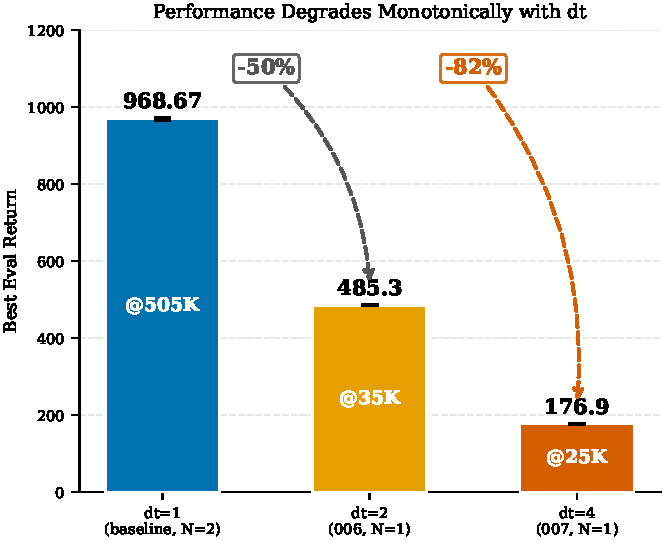
\includegraphics[width=\columnwidth]{figures/paper/fig5_dt_amplification.pdf}
\caption{Peak evaluation return as a function of imagination $\dt$. Performance degrades monotonically: $\dt{=}1$ (915.7) $>$ $\dt{=}2$ (485.3, $-47\%$) $>$ $\dt{=}4$ (176.9, $-81\%$).}
\label{fig:dt_amplification}
\end{figure}

The magnitude of degradation scales monotonically with the imagination step size (Figure~\ref{fig:dt_amplification}). From the $\dt{=}1$ baseline (915.7 at 105K), fixed $\dt{=}2$ (exp\_006) achieves a peak of only 485.3 ($-47\%$), and fixed $\dt{=}4$ (exp\_007) peaks at 176.9 ($-81\%$). This monotonic relationship is consistent with compounding model error: larger temporal gaps amplify the RSSM's prediction inaccuracy at each imagination step, and these errors accumulate across the rollout horizon.

\subsection{F5: Imagination Horizon and Subsampling Are Secondary Factors}
\label{sec:f5}

Neither horizon length nor temporal subsampling precedes collapse without multi-rate data exposure: both trained-but-unexposed configurations (008a, 008c) maintain $\nve < 0.93\times$ (\S\ref{sec:f3}), while the trained-and-exposed counterpart (008d) collapses with $\nve = 4.12\times$.  The no-embedding configurations (4 Walker seeds) show cross-seed variance (eval 140--469$^l$) but none exhibits sustained CIVO; the highest NVE ($1.69\times$, 008f s0) reflects an endpoint eval dip rather than value overestimation.

The $3.2\times$ performance gap (008a: 777.7 vs.\ 008c: 240.9) quantifies the horizon effect independently of CIVO, as both conditions maintain healthy NVE ($\leq$0.93$\times$).

% --- APPENDIX C: Full Analysis & Discussion ---

\section{Full Analysis \& Discussion}
\label{sec:appendix_analysis}

This appendix provides the complete mechanistic analysis summarized in Section~\ref{sec:discussion} of the main text. The intervention hierarchy is in Table~\ref{tab:intervention_hierarchy} (main text).

\paragraph{Fisher exact tests.}
Key pairwise comparisons (two-sided Fisher exact test): frozen (7/7 prevention) vs.\ untreated (0/10), $p < 0.001$; removed (6/6) vs.\ untreated (0/10), $p < 0.001$; wide dual-critic (3/4) vs.\ untreated (0/10), $p = 0.011$; TCN $\sigma{=}0.2$ (3/6) vs.\ untreated (0/10), $p = 0.036$; all SGS combined (1/11) vs.\ untreated (0/10), $p = 1.000$ (not significant). Only embedding removal/freezing achieves statistically significant CIVO prevention.

\subsection{The CIVO Mechanism}
\label{sec:civo_mechanism}

\begin{table}[h]
\centering
\caption{RSSM fidelity at $\dt{=}1$ vs.\ $\dt{=}2$ (v3 standardized, $N{=}600$ samples per condition). The reward prediction gap is environment-dependent: Walker trained embedding produces a $1.63\times$ reward gap, while Cheetah shows no gap ($1.00\times$) despite exhibiting CIVO. Cheetah data from a single seed.}
\label{tab:rssm_fidelity}
\footnotesize
\setlength{\tabcolsep}{4pt}
\begin{tabular}{llcccccc}
\toprule
& & \multicolumn{3}{c}{\textbf{obs\_MSE}} & \multicolumn{3}{c}{\textbf{reward\_MAE}} \\
\cmidrule(lr){3-5} \cmidrule(lr){6-8}
\textbf{Env} & \textbf{Config} & $\dt{=}1$ & $\dt{=}2$ & Gap & $\dt{=}1$ & $\dt{=}2$ & Gap \\
\midrule
\multirow{3}{*}{Walker} & Baseline & 13.49 & 27.50 & 2.04$\times$ & 0.0102 & 0.0159 & 1.56$\times$ \\
& Trained (008d) & 25.71 & 34.60 & 1.35$\times$ & 0.0530 & 0.0865 & 1.63$\times$ \\
& No emb (008f) & 8.01 & 22.04 & 2.75$\times$ & 0.7469 & 0.7526 & 1.01$\times$ \\
\midrule
Cheetah & Trained & 5.26 & 4.90 & 0.93$\times$ & 0.1410 & 0.1405 & 1.00$\times$ \\
\bottomrule
\end{tabular}
\end{table}

The RSSM fidelity analysis (Table~\ref{tab:rssm_fidelity}) reveals an environment-dependent transmission mechanism for CIVO (Figure~\ref{fig:civo_mechanism}).  On Walker Walk, the trained $\dt$-embedding produces a $1.63\times$ reward prediction gap (MAE $0.053$ at $\dt{=}1$ vs.\ $0.087$ at $\dt{=}2$), while the no-embedding configuration (008f) exhibits a $1.01\times$ gap and the baseline shows $1.56\times$, confirming that the trained embedding amplifies the fidelity discrepancy.  However, Cheetah Run shows \emph{no} reward gap ($1.00\times$, MAE ${\approx}0.141$ at both scales) despite exhibiting CIVO at $8.27\times$ NVE, indicating that reward fidelity degradation is one transmission pathway but not the only one.

In Walker, this asymmetric fidelity initiates a feedback loop with four stages: (1) the trained $\dt$-embedding causes RSSM predictions at $\dt > 1$ to carry systematically biased reward estimates; (2) the critic, trained entirely on imagined trajectories, internalizes these biased rewards as optimistic value estimates; (3) the actor exploits the overestimated regions of the value landscape, shifting its policy toward states that appear high-value only under the biased model; and (4) this policy shift further skews the distribution of imagined states, reinforcing the bias.  In Cheetah, where the reward gap is absent ($1.00\times$), CIVO must be transmitted through an alternative pathway, possibly dynamics-model prior drift in the latent state space.  In both cases, the diagnostic signature is a sustained $\nve$ above $2.0\times$, followed by evaluation collapse.

A random-policy control experiment ($N{=}100$ rollouts, 95\% bootstrap CI) decomposes CIVO into two necessary stages.  \textbf{Stage~1 (dynamics bias):} even under a random policy, $\dt{=}2$ imagination produces $1.68\times$ higher mean reward than $\dt{=}1$ in the trained-embedding model (008d): the RSSM prior already generates reward-favorable trajectories at $\dt > 1$, independent of actor behavior.  \textbf{Stage~2 (actor exploitation):} the trained actor learns to exploit these biased regions, amplifying the ratio to $2.90\times$.  In the no-embedding control (008f), neither stage is present: the random-policy ratio is $1.11\times$ and the trained-actor ratio is $0.98\times$.  The decomposition attributes $\approx 36\%$ of the total effect to dynamics bias and $\approx 64\%$ to actor exploitation, which confirms that both stages are necessary for CIVO to manifest.

This mechanism is analogous to delusional bias \citep{lu2018nondelusional}, but differs in origin: delusional bias arises from policy-class constraints, while CIVO is model-induced.  The consequence (policy exploitation of overestimated regions) is similar, but the proposed pathway is distinct.

\paragraph{Signed reward error analysis.}
To test whether CIVO arises from one-step reward overprediction, we compute signed error (predicted $-$ actual) on posterior-conditioned RSSM predictions (Table~\ref{tab:signed_error}). The trained-embedding model (008d) shows \emph{negative} bias at $\dt{=}2$ (mean signed error $-0.599$, only 8\% of samples overpredicted), ruling out observation-level reward overprediction as the mechanism. The baseline is well-calibrated (mean SE $\approx 0$), confirming methodological soundness. Value overestimation therefore occurs during \emph{imagination-level} prior drift: the RSSM prior (unconditioned on observations) generates reward-favorable trajectories at $\dt > 1$ (Stage~1 above, $1.68\times$ ratio under random policy), and the critic accumulates these into overestimated returns. The one-step reward prediction is negatively biased when conditioned on real observations, but this posterior correction is unavailable during imagination. This also distinguishes CIVO from generic compounding error, which would produce \emph{positive} signed error accumulating with horizon; the negative observation-level bias confirms that CIVO is a prior-drift phenomenon, not a reward-prediction artifact.

\begin{table}[h]
\centering
\caption{Signed reward error (predicted $-$ actual) on posterior-conditioned RSSM predictions. Negative values indicate underprediction. The trained-embedding model underpredicts at $\dt{=}2$, ruling out observation-level reward overprediction as the CIVO mechanism.}
\label{tab:signed_error}
\footnotesize
\setlength{\tabcolsep}{4pt}
\begin{tabular}{llrrrrr}
\toprule
\textbf{Config} & $\dt$ & \textbf{Mean SE} & \textbf{Std} & \textbf{\%Over} & \textbf{Actual} & \textbf{Pred} \\
\midrule
Baseline & 1 & $+0.001$ & 0.023 & 39.6\% & 1.893 & 1.894 \\
\midrule
008d (trained) & 1 & $+0.018$ & 0.072 & 61.8\% & 0.361 & 0.379 \\
008d (trained) & 2 & $\mathbf{-0.599}$ & 0.722 & 8.0\% & 0.721 & 0.121 \\
\midrule
008f (no emb) & 1 & $-0.710$ & 0.704 & 14.0\% & 0.921 & 0.211 \\
008f (no emb) & 2 & $-1.645$ & 1.485 & 5.0\% & 1.840 & 0.195 \\
\bottomrule
\end{tabular}
\end{table}

\paragraph{Embedding geometry (exp\_065).}
To characterize what the trained $\dt$-embedding learns, we measure pairwise cosine similarity between $e_{\dt{=}1}$ and $e_{\dt{=}2}$ across training checkpoints for three trained seeds (two environments) and two frozen controls (Table~\ref{tab:cosine_sim}).

\begin{table}[h]
\centering
\caption{Cosine similarity between $e_{\dt{=}1}$ and $e_{\dt{=}2}$ vectors. Trained embeddings converge to near-opposite representations; frozen embeddings remain near-orthogonal throughout.}
\label{tab:cosine_sim}
\footnotesize
\setlength{\tabcolsep}{4pt}
\begin{tabular}{llrrr}
\toprule
\textbf{Config} & \textbf{Env} & \textbf{cos@25K} & \textbf{cos@75K} & \textbf{Status} \\
\midrule
008d s3 (trained) & Walker & $-0.87$ & $-0.70$ & CIVO \\
059 s5 (trained) & Walker & $-0.94$ & $-0.86$ & CIVO \\
010b s0 (trained) & Cheetah & $-0.90$ & $-0.84$ & CIVO \\
\midrule
057 s2 (frozen) & Walker & $-0.15$ & $-0.15$ & Healthy \\
058 s1 (frozen) & Cheetah & $+0.07$ & $+0.07$ & Healthy \\
\bottomrule
\end{tabular}
\end{table}

All trained seeds map $\dt{=}1$ and $\dt{=}2$ to nearly opposite directions (cosine similarity $-0.70$ to $-0.94$), consistent across both Walker and Cheetah environments. Frozen controls remain near-orthogonal (cosine $\approx 0$) and constant across all checkpoints. The full pairwise cosine similarity matrix (Figure~\ref{fig:pairwise_heatmap}) reveals that the near-antipodal relationship between $e_{\dt{=}1}$ and $e_{\dt{=}2}$ is the dominant structure: most other $\dt$-pairs remain near-orthogonal ($|\text{cos}| < 0.2$). The RSSM selectively maximizes separation along the $\dt{=}1$ vs.\ $\dt{=}2$ axis rather than learning a globally structured embedding space.

\begin{figure}[h]
\centering
\includegraphics[width=0.55\columnwidth]{figures/paper/pairwise_heatmap.png}
\caption{Pairwise cosine similarity between all $\dt$-embedding vectors (exp\_008d, seed 3, step 75K). The $e_{\dt{=}0}$--$e_{\dt{=}1}$ pair exhibits strong anti-correlation ($-0.70$); remaining pairs are near-orthogonal. The learned geometry is dominated by a single antipodal axis.}
\label{fig:pairwise_heatmap}
\end{figure}

The magnitude of the learned separation, near-antipodal rather than merely distinct, provides converging evidence that the RSSM develops maximally differentiated internal representations for the two temporal scales, which in turn may contribute to the asymmetric reward fidelity gap reported in Table~\ref{tab:rssm_fidelity} and replicated below.

\paragraph{Extended RSSM fidelity replication (exp\_063).}
To validate the fidelity gap on independently trained checkpoints, we repeat the posterior-conditioned analysis with 15 episodes $\times$ 40 test points $\times$ 4 $\dt$ levels (600 samples per model) on final checkpoints from three conditions (Table~\ref{tab:rssm_fidelity_ext}).

\begin{table}[h]
\centering
\caption{RSSM fidelity analysis on Walker Walk (training-time posterior-conditioned, pre-v3 standardization). Reward prediction gap magnitude varies across checkpoints and measurement protocols: this posterior-conditioned analysis yields $3.11\times$, while v3 standardized analysis (Table~\ref{tab:rssm_fidelity}) yields $1.63\times$. The qualitative pattern, that the trained embedding amplifies the reward gap while improving observation reconstruction, is consistent across both.}
\label{tab:rssm_fidelity_ext}
\footnotesize
\setlength{\tabcolsep}{4pt}
\begin{tabular}{lcccccc}
\toprule
& \multicolumn{3}{c}{\textbf{obs\_MSE}} & \multicolumn{3}{c}{\textbf{reward\_MAE}} \\
\cmidrule(lr){2-4} \cmidrule(lr){5-7}
\textbf{Config} & $\dt{=}1$ & $\dt{=}2$ & Gap & $\dt{=}1$ & $\dt{=}2$ & Gap \\
\midrule
Baseline (009d) & 16.08 & 23.49 & 1.46$\times$ & 0.045 & 0.059 & 1.30$\times$ \\
Collapsed (008d) & 9.96 & 13.21 & 1.33$\times$ & 0.057 & 0.178 & 3.11$\times$ \\
Frozen (057) & 11.14 & 14.95 & 1.34$\times$ & 0.068 & 0.133 & 1.96$\times$ \\
\bottomrule
\end{tabular}
\end{table}

The posterior-conditioned replication confirms the qualitative fidelity gap pattern on Walker with two additional observations. First, the collapsed model achieves the \emph{lowest} absolute obs\_MSE at $\dt{=}1$ (9.96 vs.\ baseline 16.08), indicating that the trained $\dt$-embedding improves world model quality overall; the pathology is selective degradation of reward predictions at longer horizons, not general model failure. Second, freezing the $\dt$-embedding reduces the reward gap from $3.11\times$ to $1.96\times$, providing converging evidence for its role in preventing the co-adaptation loop. The magnitude difference between this posterior-conditioned analysis ($3.11\times$) and the v3 standardized result ($1.63\times$, Table~\ref{tab:rssm_fidelity}) reflects checkpoint and protocol variation; the directional pattern is robust.

\paragraph{Value prediction analysis (exp\_064).}
To examine the relationship between RSSM reward fidelity and critic value estimates, we compare critic predictions $V(s)$ against actual evaluation returns across three conditions (Table~\ref{tab:value_pred}).

\begin{table}[h]
\centering
\caption{Critic value predictions vs.\ actual evaluation returns. The CIVO model's critic is well-calibrated to its $\lambda$-return targets ($V(s) \approx$ target) but both $V$ and targets are disconnected from reality (VE${=}3.03\times$).}
\label{tab:value_pred}
\footnotesize
\setlength{\tabcolsep}{4pt}
\begin{tabular}{lrrrr}
\toprule
\textbf{Config} & $V(s)$ & \textbf{Eval} & \textbf{VE ratio} & $V{-}\text{target}$ \\
\midrule
Baseline (001) & 665.9 & 938.9 & 0.71$\times$ & $+0.001$ \\
CIVO (008d) & 192.7 & 63.6 & \textbf{3.03}$\times$ & $+0.586$ \\
No emb (008f) & 116.5 & 306.5 & 0.38$\times$ & $+0.316$ \\
\bottomrule
\end{tabular}
\end{table}

\begin{figure}[h]
\centering
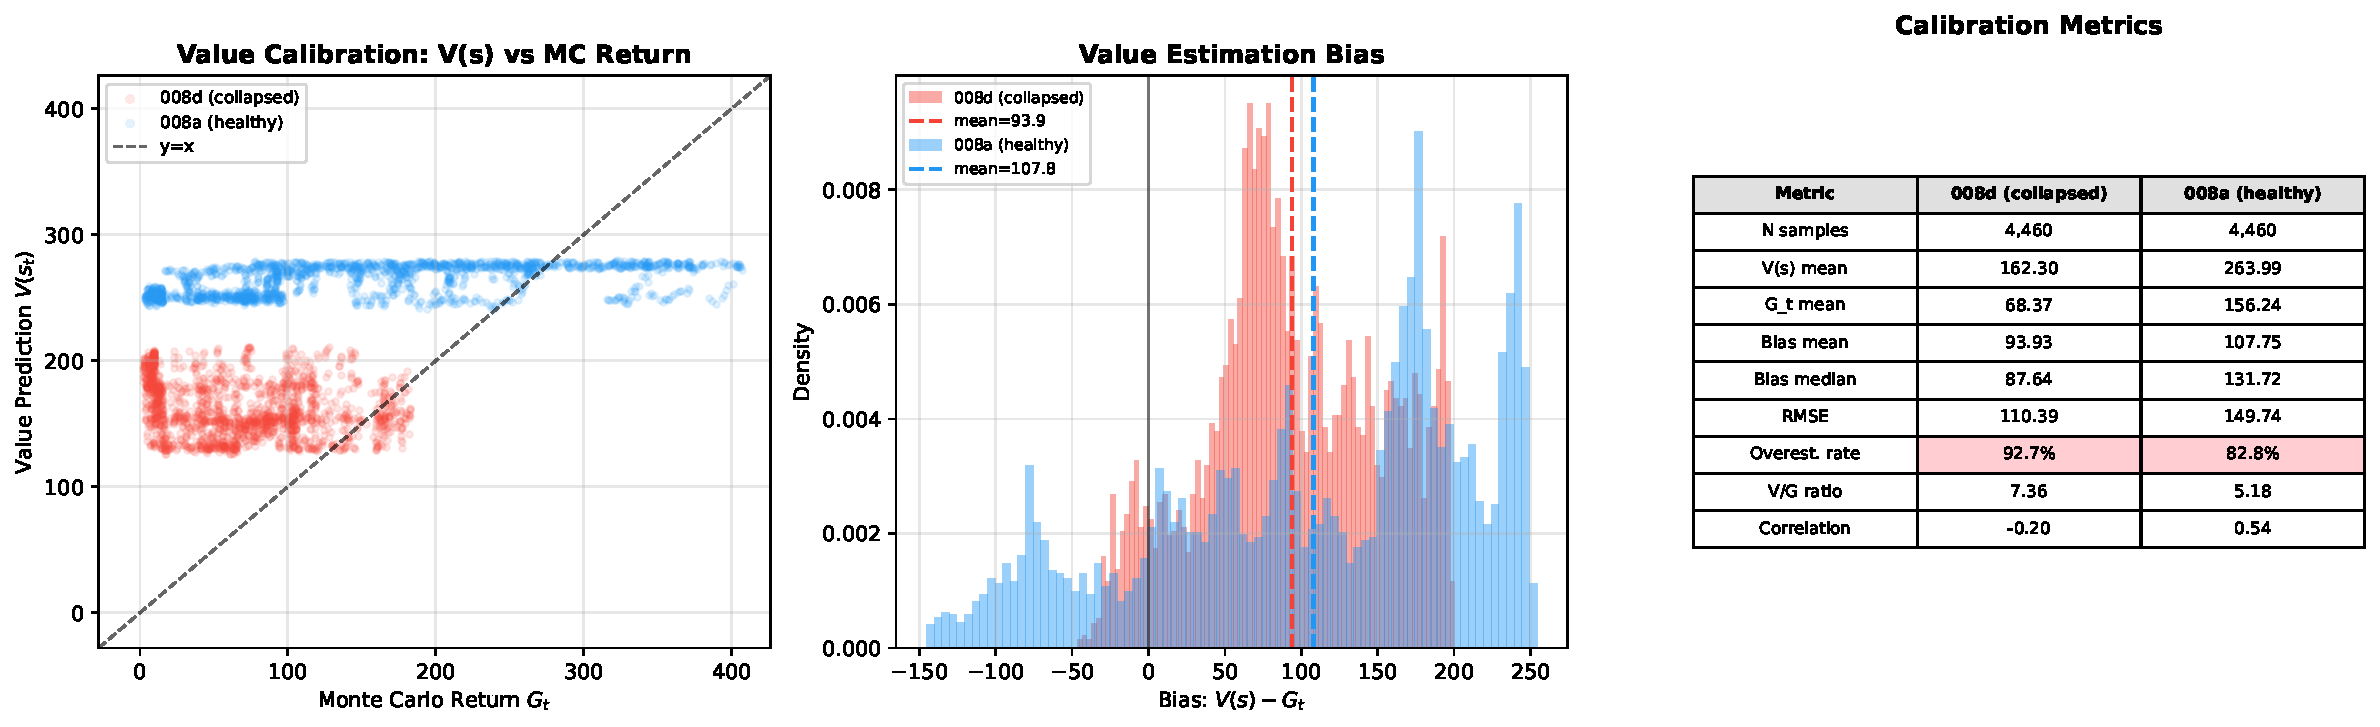
\includegraphics[width=0.85\columnwidth]{figures/value_vs_returns.pdf}
\caption{Critic value $V(s)$ vs.\ episodic return $G_t$ for collapsed (008d, left) and healthy (008a, right) configurations. The collapsed critic's predictions are \emph{negatively} correlated with actual returns ($r = {-}0.20$), indicating delusional value ranking: states assigned higher value actually produce \emph{lower} returns. The healthy critic maintains positive correlation ($r = {+}0.54$) despite comparable overestimation rates (92.7\% vs.\ 82.8\%), demonstrating that bias magnitude is not the distinguishing pathology; value-return \emph{ordering} is.}
\label{fig:value_vs_returns}
\end{figure}

The correlation analysis (Figure~\ref{fig:value_vs_returns}) reveals a critical distinction: bias alone does not differentiate CIVO pathology from normal value estimation error: both collapsed and healthy critics overestimate (92.7\% vs.\ 82.8\% of states). The pathological signature is \emph{delusional ranking}: the collapsed critic's $V(s)$ is negatively correlated with actual returns ($r = {-}0.20$), meaning it systematically directs the actor toward low-return regions of state space. The healthy critic, while biased, preserves ordinal accuracy ($r = {+}0.54$), allowing the actor to make directionally correct decisions.

The paradox, that $V(s)$ tracks its $\lambda$-return targets faithfully yet overestimates actual performance by $3\times$, provides converging evidence for the hypothesized mechanism in which CIVO operates upstream of the critic: the world model generates inflated imagination trajectories that the critic learns faithfully, producing targets disconnected from reality. In the baseline, VE${<}1.0$ throughout training because $V(s)$ reflects discounted imagined returns over $H{=}15$ steps, naturally lower than undiscounted episodic evaluation. The CIVO model crosses VE${=}1.0$ at step 55K and reaches $3.03\times$ by 105K, with the gap widening as the actor exploits the overoptimistic critic.

\paragraph{Actor entropy dynamics under CIVO.}
Extended training of collapsed configurations reveals a distinctive temporal sequence: evaluation return collapses first, followed by actor entropy explosion ${\sim}35$K steps later. In the most severe case (collapsed seed~A), entropy rises from $-5.21$ to $+3.22$ nats at a rate of $+2.11$ nats/10K steps, with returns declining from 583 to 93 between steps 60K--120K. A second collapsed run (collapsed seed~B) shows $+0.61$ nats/10K with comparable return degradation (583$\to$102). By contrast, healthy baselines exhibit gradual entropy drift at $+0.07$ to $+0.22$ nats/10K, 15--30$\times$ slower, with returns stable above 900. The return-before-entropy temporal ordering is consistent with the causal chain: delusional critic $\to$ bad actor gradients $\to$ policy destabilization. The entropy explosion is a lagging indicator; the NVE diagnostic detects CIVO onset ${\sim}35$K steps before entropy rises, consistent with its use as an early-warning signal (\S\ref{sec:appendix_sensitivity}).

\subsection{Selective Gradient Stopping and Gradient Decomposition}
\label{sec:sgs_gradient_analysis}

\subsubsection{Gradient Decomposition Results}
\label{sec:gradient_decomposition}

\begin{figure}[t]
\centering
\includegraphics[width=0.75\columnwidth]{figures/fig3_gradient_decomposition.pdf}
\caption{Gradient contribution to $e_{\Delta t}$ by loss component at two training checkpoints. The reward head contributes the largest share (38--49\%) yet reward-only SGS (exp\_016e) fails; the observation decoder channel (16--22\%) carries the critical $\dt$-specific spatial information that drives the RSSM fidelity gap.}
\label{fig:gradient_decomp}
\end{figure}

Exp\_016e collapses in the same qualitative pattern as the unmodified control: peak evaluation 326.7 at 75K steps followed by catastrophic decline to 31.7 at 95K, with NVE reaching $10.42\times$. The SGS intervention neither prevented nor attenuated CIVO.

To explain this null result, we performed a gradient decomposition analysis using \texttt{torch.autograd.grad} to measure each loss component's contribution to $\nabla_\theta e_{\Delta t}$, where $\theta$ denotes the temporal embedding parameters. Table~\ref{tab:gradient_decomposition} reports the results.

\begin{table}[ht]
\centering
\caption{Gradient contributions to the temporal embedding $e_{\Delta t}$ by loss component, measured via \texttt{torch.autograd.grad} with training configuration \texttt{gate\_fixed\_dt=2}. Gradient norms are $\ell_2$ norms of $\nabla_\theta \mathcal{L}_i$ for each loss $\mathcal{L}_i$.}
\label{tab:gradient_decomposition}
\small
\begin{tabular}{lrrrr}
\toprule
& \multicolumn{2}{c}{\textbf{@55K}} & \multicolumn{2}{c}{\textbf{@112K}} \\
\cmidrule(lr){2-3} \cmidrule(lr){4-5}
Loss component & Share & (\%) & Share & (\%) \\
\midrule
Reward head & --- & 49.0 & --- & 38.1 \\
KL dynamics & --- & 34.7 & --- & 40.4 \\
Observation decoders & --- & 16.3 & --- & 21.5 \\
\bottomrule
\end{tabular}
\end{table}

The gradient decomposition reveals a counterintuitive structure: the reward head provides the largest gradient contribution (49.0\% at 55K, 38.1\% at 112K), yet reward-only SGS (exp\_016e) fails catastrophically (NVE $10.42\times$). The observation decoder channel contributes the smallest share (16.3\% at 55K, 21.5\% at 112K) yet carries the critical $\dt$-specific spatial information.  This dissociation between gradient magnitude and causal importance explains why exp\_016e, which targets the largest pathway, is functionally insufficient for CIVO prevention.

The gradient structure is relatively stable across training (reward shifts from 49\% to 38\%, obs from 16\% to 22\%, KL from 35\% to 40\%), unlike what a magnitude-based account would predict. The reward head's large gradient contribution reflects the scalar reward prediction task's sensitivity to temporal embedding parameters, but this gradient does not encode $\Delta t$-specific structural information about spatial dynamics. The observation decoder channel, despite its smaller magnitude, is the only pathway that encodes how the RSSM should differentially predict multi-dimensional proprioceptive states across temporal scales.

\paragraph{Why the smallest channel is causally critical.} The observation decoder is the only loss component whose gradients encode how the RSSM should differentially predict multi-dimensional proprioceptive states ($14$ orientations, $9$ velocities, $1$ height) across temporal scales.  This $\dt$-specific spatial information shapes the latent state representation in ways that propagate to reward prediction: the RSSM fidelity gap (Walker: $1.63\times$ reward MAE ratio, Table~\ref{tab:rssm_fidelity}) arises because the temporal embedding learns to produce latent states that are spatially biased at $\dt{>}1$, not because the reward head directly learns scale-dependent biases.  Full-SGS targets this causal chain by preventing observation-decoder gradients from updating $e_{\Delta t}$, though its 0/2 CIVO elimination rate on Walker (seed~1: NVE reduced from $4.12\times$ to $1.66\times$ but remains CIVO-positive; seed~2: collapsed) indicates that breaking the gradient pathway alone does not fully eliminate the vulnerability.

\subsubsection{Implications for the CIVO Mechanism}
\label{sec:sgs_implications}

The gradient decomposition reveals that gradient magnitude and pathway importance are decoupled in CIVO.

\paragraph{Gradient importance $\neq$ gradient magnitude.} The reward head contributes the largest gradient share (38--49\%) to $e_{\Delta t}$, yet reward-only SGS fails.  The observation decoder contributes the smallest share (16--22\%), yet its removal (via Full-SGS) is necessary for CIVO mitigation.  This dissociation arises because the reward head's gradient, while large, does not encode $\dt$-specific structural information: it adjusts $e_{\Delta t}$ to minimize a scalar prediction error that is largely $\dt$-invariant.  The observation decoder's gradient, though smaller, encodes how the RSSM should differentially reconstruct 24-dimensional proprioceptive states across temporal scales. This is the channel through which $e_{\Delta t}$ learns scale-dependent latent biases.

\paragraph{Reframing the intervention target.} Any gradient-level strategy that targets the reward head alone (reward prediction regularization, reward-conditioned value clipping, or reward-only SGS) targets the largest pathway but not the informationally critical one.  The failure of exp\_016e (NVE $10.42\times$) despite detaching the dominant gradient source confirms this.  Full-pathway SGS (exp\_018) detaches $e_{\Delta t}$ from all non-KL gradients, retaining only the KL dynamics contribution (34--40\%).  However, this intervention eliminates CIVO in neither seed: seed~1 shows partial mitigation (eval 448.3, peak NVE $1.66\times$, still CIVO-positive) while seed~2 collapses (eval 40.8). Removing the observation decoder gradient channel is thus contributory but not sufficient. Figure~\ref{fig:civo_decomposition} decomposes evaluation returns across conditions.

\begin{figure}[ht]
\centering
\includegraphics[width=0.75\columnwidth]{figures/fig2_civo_decomposition.pdf}
\caption{CIVO decomposition: peak and final (105K step) evaluation returns on Walker Walk across four conditions. \textbf{Baseline} (001): vanilla DreamerV3. \textbf{Trained dt-emb} (008d)\protect\footnotemark: learned $d{=}32$ temporal embedding with multi-rate data. \textbf{Full-SGS} (s1, s2): trained embedding with all non-KL gradients detached from $e_{\dt}$. Trained $\dt$-embedding degrades peak eval by $73\%$ and final eval by $86\%$. Full-SGS seed~1 shows partial mitigation ($-51\%$ final, NVE $1.66\times$, still CIVO-positive) while seed~2 collapses ($-96\%$ final). CIVO elimination rate $= 0/2$.}
\label{fig:civo_decomposition}
\end{figure}
\footnotetext{Experiment 008d terminated at 55K steps; the 105K data point uses continuation run 009e under identical configuration.}

Cross-environment validation on Cheetah Run (exp\_021) further clarifies the role of Full-SGS.  The intervention did not prevent the initial CIVO onset: NVE peaked at $9.94\times$ at 45K (comparable to the unmitigated exp\_010b's $8.27\times$).  However, unlike exp\_010b, which collapsed permanently to eval 51.7, exp\_021 self-corrected within ${\sim}$10K steps, with sustained NVE dropping to $0.34\times$ (55K--105K) and final evaluation recovering to 221.5.  This transient self-correcting trajectory is not attributable to the SGS intervention: the initial CIVO onset and peak severity are comparable to the unmitigated case, and the self-correction may reflect Cheetah Run's simpler dynamics rather than SGS efficacy.  Performance remains at 38.7\% of baseline (572.5), likely because Full-SGS over-aggressively blocks actor gradients (actor gradient norms near zero throughout training).  Combined with exp\_018's Walker results (0/2 CIVO elimination), these findings yield a 0/3 elimination rate across environments, indicating that gradient-level interventions alone do not eliminate the CIVO vulnerability. Additional mechanisms (e.g., forward-pass conditioning effects, residual capacity-dependent instabilities) operate beyond the gradient pathway.

\paragraph{Connection to RSSM fidelity analysis.} The trained-embedding condition on Walker (exp\_008d) shows a $1.63\times$ reward gap between $\Delta t{=}1$ and $\Delta t{=}2$ transitions (Table~\ref{tab:rssm_fidelity}); Cheetah shows no gap ($1.00\times$) despite exhibiting CIVO, indicating environment-dependent transmission.  This gap arises because the observation decoder gradients shape $e_{\Delta t}$ to produce latent states that are spatially biased at $\dt{>}1$, and the reward head inherits these biases \textit{through the latent state} rather than learning them directly.  The reward head's large gradient contribution reflects sensitivity to $e_{\Delta t}$'s parameters but not causal responsibility for the fidelity gap.

\subsubsection{Entropy Dynamics Across Configurations}
\label{sec:entropy_dynamics}

\begin{figure}[ht]
\centering
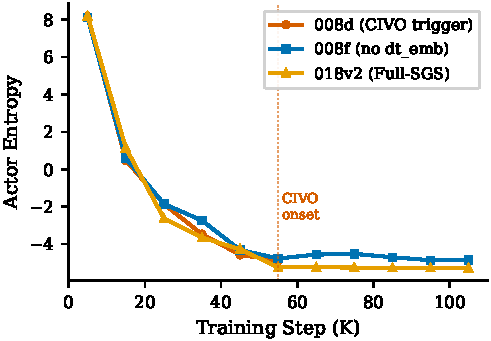
\includegraphics[width=0.85\columnwidth]{figures/fig4_entropy_dynamics.pdf}
\caption{Actor entropy trajectories for three configurations. All start at ${\sim}8$ nats and converge to similar values (${\sim}{-}4.5$ to ${-}5$). The CIVO-triggering configuration (008d, red) follows a normal entropy reduction trajectory; the divergence from the control (008f) is subtle in entropy space, consistent with CIVO operating through the value channel rather than the entropy channel. 018v2 (Full-SGS, seed~1) shows slightly lower terminal entropy.}
\label{fig:entropy_dynamics}
\end{figure}

\subsubsection{Exp\_016e Reinterpreted as Stochastic Variation}
\label{sec:016e_reinterp}

The gradient decomposition establishes that exp\_016e targets the largest gradient pathway (reward: 38--49\%) but not the informationally critical one (observation decoders: 16--22\%).  The apparent timing differences between exp\_016e and exp\_008d (later collapse onset, 75K vs.\ 25K, and higher peak evaluation, 326.7 vs.\ 167.2) must be attributed to stochastic variation rather than SGS effects, since the critical observation decoder channel remains intact.  Two of three trajectories (exp\_008d, exp\_016e) cross the $2.0\times$ diagnostic threshold (peak NVE $4.12\times$ and $10.42\times$ respectively); exp\_009b peaks at $1.62\times$ (sub-threshold under $\tau{=}2.0$) and self-corrects, consistent with the stochastic onset pattern identified in \S\ref{sec:seed_divergence}.

\subsection{Post-CIVO Outcomes: Why Seeds Diverge}
\label{sec:seed_divergence}

\begin{table}[ht]
\centering
\caption{Post-CIVO outcomes for all six runs exceeding the $\nve \geq 2.0\times$ diagnostic threshold across two environments. Peak/Final NVE measured in the 35K+ window.}
\label{tab:post_civo}
\footnotesize
\setlength{\tabcolsep}{3pt}
\begin{tabular}{llcccl}
\toprule
\textbf{Env} & \textbf{Seed} & \textbf{Peak} & \textbf{Final} & \textbf{Eval} & \textbf{Outcome} \\
\midrule
Walker & s1 (008d) & 4.12$\times$ & 4.12$\times$ & 82.8 & Full collapse \\
Walker & s4 (008d\_s4) & 4.62$\times$ & 4.62$\times$ & 63.6 & Full collapse \\
Walker & s5 (059) & 4.72$\times$ & 1.22$\times$ & 95.8 & Collapse$^\dagger$ \\
\midrule
Cheetah & s1 (010b) & 8.27$\times$ & 8.27$\times$ & 51.7 & Full collapse \\
Cheetah & s0 (078) & 4.10$\times$ & 0.29$\times$ & 119.5 & Self-correcting$^\ddagger$ \\
Cheetah & s0 (010b\_s0) & 108.52$\times$ & 108.52$\times$ & 0.83 & Full collapse \\
\bottomrule
\end{tabular}
\vspace{1pt}
{\raggedright\footnotesize Two sub-threshold runs (009b, peak $1.62\times$; 008d\_s3, peak $1.53\times$) are omitted. $^\dagger$~NVE self-corrected ($4.72\times$ $\to$ $1.22\times$) but policy did not recover (eval 10.5\% of baseline). $^\ddagger$~Peak NVE $4.10\times$ at 75K; eval 213.7$\to$26.1$\to$119.5 (26.8\% of 2-seed baseline mean, 446.1).\par}
\end{table}

All six runs in Table~\ref{tab:post_civo} exceed the $\nve \geq 2.0\times$ diagnostic threshold, yet the downstream damage is stochastic.\footnote{Exp\_009e was excluded from multi-seed analyses due to a seed configuration error (default seed=0, identical to exp\_008d).}  Sustained collapse is the majority outcome (4/6 runs). One run self-corrects (Cheetah exp\_078, recovering from 26.1 to 119.5 at 105K); one (Walker seed~5, exp\_059) shows NVE self-correction ($4.72\times \to 1.22\times$) but the policy remains collapsed (eval 10.5\% of baseline). Cheetah seed~1 (010b) exhibits more extreme overestimation (peak NVE $8.27\times$) than Walker seeds ($4.12$--$4.72\times$), consistent with the Cheetah reward scale amplifying the fidelity gap.  We hypothesize that the divergence relates to the critic's representational capacity at the time of CIVO onset.  \citet{lyle2022capacity} demonstrate that deep RL networks suffer progressive capacity loss, in which early-learned features become increasingly difficult to overwrite.  If the critic's capacity is already partially consumed when CIVO injects overestimation, the network cannot recalibrate (e.g., 008d); if sufficient capacity remains, the critic can absorb transient overestimation and recover (e.g., 078).

\paragraph{A fourth trajectory: CIVO-induced persistent value collapse.}
Obs-decoder SGS seed~3 (exp\_025) exhibits a trajectory not observed in the untreated seeds: healthy through 105K ($\nve < 1.0\times$, eval 818.6), CIVO onset at 135K ($\nve = 5.47\times$, eval 67.0), followed by evaluation recovery (590.2 at 215K, 64\% of baseline) but persistent value collapse ($\nve = 0.14\times$, value mean 80.6). The critic undershoots after the CIVO episode, suggesting that CIVO-induced representational damage persists even when the policy partially recovers. This contrasts with sub-threshold transient overestimation (009b, peak $1.62\times$), where both value and evaluation recover jointly, and with full collapse (seed~1, 008d), where neither recovers. Seed~4 exhibits the same terminal value collapse ($\nve = 0.14\times$ at 215K, eval 242), suggesting this overcorrection is systematic rather than seed-specific. The pattern adds a fourth post-CIVO outcome, policy recovery with critic damage, to the three documented in Table~\ref{tab:post_civo}.

\subsubsection{Failure and Degradation Mode Taxonomy}

Table~\ref{tab:failure_modes} classifies the six distinct failure and degradation modes observed across all experimental configurations. The taxonomy reveals that CIVO is not a single failure mode but a family of related pathologies, with the trained $\dt$-embedding creating vulnerability through at least two independent mechanisms: value-driven collapse (monotonic, late-onset, and SGS-resistant CIVO) and gradient-mediated effects (gradient starvation, SGS-paradoxical worsening).

\begin{table}[ht]
\centering
\caption{Failure and degradation mode taxonomy. Each mode is characterized by its NVE trajectory, entropy behavior, and primary mechanism.}
\label{tab:failure_modes}
\footnotesize
\setlength{\tabcolsep}{3pt}
\begin{tabular}{@{}llccl@{}}
\toprule
\textbf{Mode} & \textbf{Representative} & \textbf{NVE} & \textbf{Entropy} & \textbf{Mechanism} \\
\midrule
Monotonic CIVO & 008d, 008d\_s4, 010b\_s0 & $\uparrow$ sustained & $\downarrow$ & Reward bias $\to$ critic $\to$ actor \\
Late-onset CIVO & 008d\_s3 & $\uparrow$ delayed & $\downarrow$ & Same, delayed onset \\
Transient CIVO & 009b & Peak $\to$ $\downarrow$ & Stable & Self-correction via capacity \\
Grad.\ starvation & 015b & Oscillates, decays & Stable & Frozen emb $\to$ zero actor grad \\
SGS-resistant & 018\_s2 & $\uparrow$ & $\downarrow$ & Forward-pass conditioning \\
SGS-paradoxical & 016e & $\uparrow$ sustained & $\downarrow$ & Reward SGS $\to$ obs-dec reliance \\
\bottomrule
\end{tabular}
\end{table}

\subsection{Extended Training Dynamics}\label{sec:extended_training}

One Walker seed (s3, exp\_045) was extended from 112K to approximately 302K steps to investigate long-horizon CIVO dynamics. After onset (NVE peak $4.91\times$ at 132K steps), the system exhibited complete self-recovery: NVE declined to $0.05\times$ and evaluation performance recovered to 867.6 (94.7\% of baseline). This recovery required approximately 170K additional training steps beyond onset. The trajectory shows a single onset--recovery cycle with no recurrence, suggesting that the CIVO feedback loop can break spontaneously given sufficient training, though at substantial computational cost that the frozen $\dt$-embedding diagnostic eliminates entirely.

\subsection{Why MPC Is Immune}
\label{sec:mpc_immune}

\citet{nhu2025tawm} show that $\dt$-conditioning benefits TD-MPC2, raising the question of why it fails in DreamerV3.  The critical difference is that MPC re-plans from real states at every step, so imagination errors do not accumulate into the training signal because there is no critic bootstrapping from imagined trajectories.  In DreamerV3, the actor-critic trains entirely within imagination, and any systematic reward-prediction bias at $\dt > 1$ is amplified through the closed actor-critic loop.

\subsection{The \texorpdfstring{$\dt$}{dt}-Embedding Dilemma}
\label{sec:embedding_dilemma}

The factorial results reveal a fundamental tension: removing the $\dt$-embedding (008f) eliminates CIVO but at a $14\times$ cost to reward prediction quality ($0.7469$ vs.\ $0.0530$ MAE), as the world model cannot distinguish temporal scales.  Restricting imagination to $\dt{=}1$ while retaining the trained embedding (008e\_v3) eliminates CIVO entirely (all four seeds show NVE $\leq 0.8\times$, well below the $2.0\times$ threshold), with three of four seeds achieving $64$--$94\%$ of baseline performance (mean $775.6$; \S\ref{sec:f6}).  This confirms that multi-step imagination at $\dt > 1$ is necessary for CIVO induction; the trained embedding alone is insufficient.

\subsection{Temporal Embedding Representation Analysis}
\label{sec:cosine_evolution}

To understand how the trained $\dt$-embedding creates vulnerability, we analyze the cosine similarity between $e(\dt{=}1)$ and $e(\dt{=}2)$ across training (exp\_065). Trained embeddings learn \emph{near-opposite} representations: $\cos(e_1, e_2) = {-}0.87$ to ${-}0.94$ at 25K steps across three configurations (Walker 008d\_s3, Cheetah 010b\_s0, Walker 059\_s5), persisting at ${-}0.70$ to ${-}0.86$ at 75K steps (Figure~\ref{fig:cosine_similarity}). In contrast, frozen embeddings maintain near-zero similarity ($-0.15$ to $+0.07$, constant throughout training), and untrained embeddings show effectively zero differentiation ($\cos = +0.024$). The near-antipodal learned representations explain the large reward prediction gap (\S\ref{sec:f2}): $\dt{=}2$ conditioning pushes the RSSM into a qualitatively different region of latent space, producing systematically biased predictions rather than minor perturbations.

\begin{figure}[h]
\centering
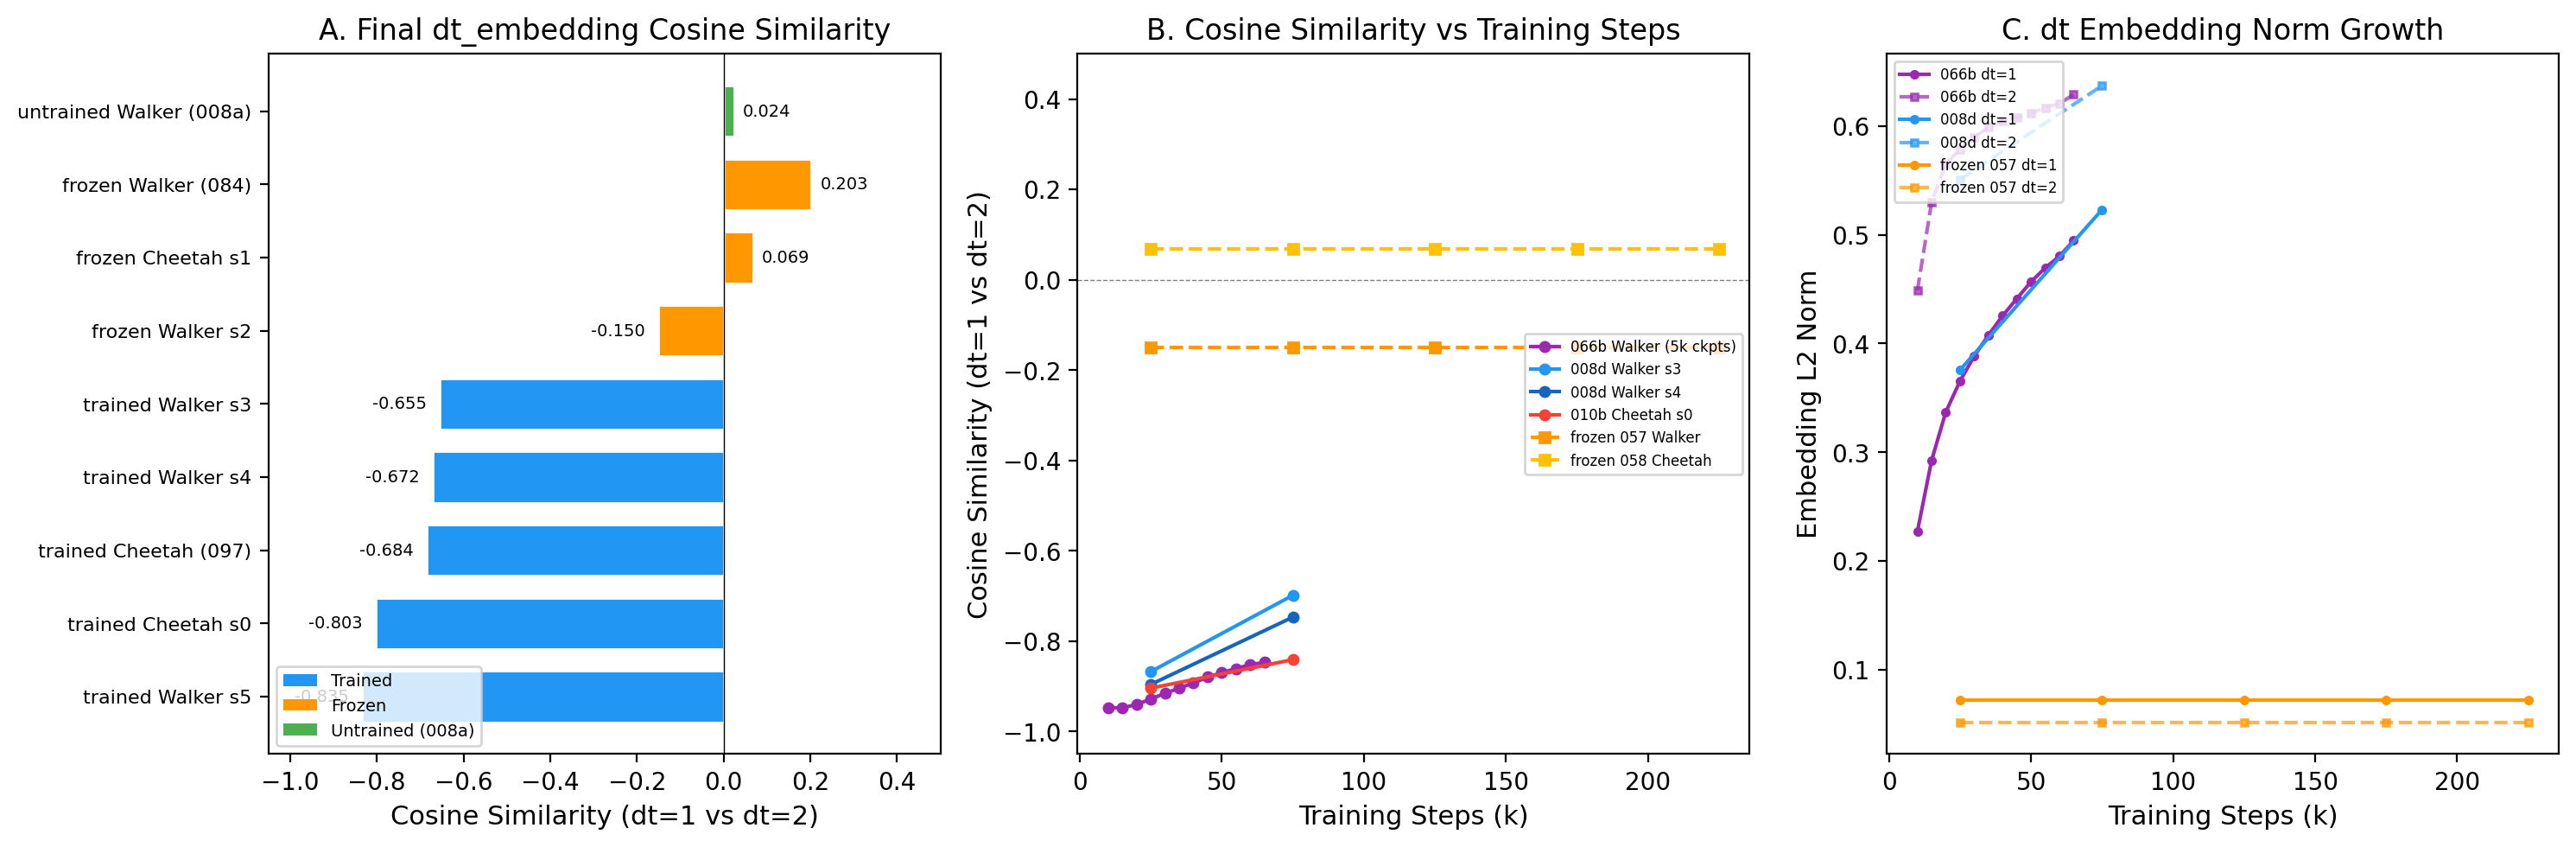
\includegraphics[width=0.85\columnwidth]{figures/dt_embedding_cosine_similarity.png}
\caption{Cosine similarity between $e(\dt{=}1)$ and $e(\dt{=}2)$ across training configurations. Trained $\dt$-embeddings (Walker and Cheetah) rapidly converge to near-antipodal representations ($\cos \in [{-}0.65, {-}0.90]$), while frozen and untrained embeddings remain near zero throughout training. The anti-correlation emerges within the first 25K steps, coinciding with the CIVO onset window (\S\ref{sec:cosine_temporal}). This provides the representation-level smoking gun: trained gradient flow drives the embedding to encode $\dt{=}1$ and $\dt{=}2$ as maximally differentiated directions, creating the asymmetric latent space that underlies RSSM prediction bias.}
\label{fig:cosine_similarity}
\end{figure}

\subsection{\texorpdfstring{$\dt$}{dt}-Embedding Differentiation Precedes Value Divergence}
\label{sec:cosine_temporal}

The preceding analysis established that trained $\dt$-embeddings learn near-antipodal representations. Here we resolve the \emph{temporal dynamics} of this differentiation across 11 experiments (${\sim}$47 checkpoints), testing whether embedding differentiation is a consequence or precursor of CIVO.

\paragraph{Trained embeddings: monotonic relaxation.}
Across all trained configurations, $\cos(e_1, e_2)$ starts near $-0.95$ within 10K steps and relaxes monotonically toward ${\sim}{-}0.65$ (Table~\ref{tab:cosine_evolution_ext}).

\begin{table}[h]
\centering
\caption{Cosine similarity evolution between $e(\dt{=}1)$ and $e(\dt{=}2)$ for trained $\dt$-embeddings. Relaxation is monotonic but never reaches zero; frozen embeddings remain constant near zero throughout training.}
\label{tab:cosine_evolution_ext}
\footnotesize
\setlength{\tabcolsep}{4pt}
\begin{tabular}{llccccc}
\toprule
\textbf{Env} & \textbf{Experiment} & \textbf{10K} & \textbf{25K} & \textbf{65K} & \textbf{75K} & \textbf{302K} \\
\midrule
\multirow{2}{*}{Walker} & exp\_066b (trained) & $-0.947$ & $-0.928$ & $-0.847$ & --- & --- \\
 & exp\_045 (extension) & --- & --- & --- & --- & $-0.668$ \\
\midrule
Cheetah & exp\_010b$\to$048 & --- & $-0.904$ & --- & $-0.841$ & $-0.639$ \\
\midrule
\multicolumn{2}{l}{\textit{Frozen controls:}} \\
Walker & exp\_057 (frozen) & \multicolumn{5}{c}{$-0.150$ (constant, 25K--225K)} \\
Cheetah & exp\_058 (frozen) & \multicolumn{5}{c}{$+0.069$ (constant, 25K--225K)} \\
\bottomrule
\end{tabular}
\end{table}

Cross-seed consistency at 25K steps is high: mean $\cos = -0.910 \pm 0.028$ ($n{=}5$ Walker seeds), confirming the relaxation pattern is robust across random seeds. Variance increases with training ($-0.789 \pm 0.076$ at 75K), reflecting seed-dependent relaxation rates.

\paragraph{Temporal precedence over CIVO.}
Exp\_066b provides simultaneous cosine similarity and CIVO diagnostic data at 5K resolution (Table~\ref{tab:cosine_vs_civo}).

\begin{table}[h]
\centering
\caption{Cosine similarity relaxation and CIVO diagnostic for exp\_066b. Embedding relaxation onset (${\sim}$20K) precedes CIVO alert (55K, VE ratio $> 0.7$) by ${\sim}$30--35K steps.}
\label{tab:cosine_vs_civo}
\footnotesize
\setlength{\tabcolsep}{5pt}
\begin{tabular}{rccc}
\toprule
\textbf{Step} & $\cos(e_1, e_2)$ & \textbf{VE ratio} & \textbf{CIVO alert} \\
\midrule
10K & $-0.947$ & 0.012 & --- \\
15K & $-0.948$ & 0.033 & --- \\
25K & $-0.928$ & 0.193 & --- \\
35K & $-0.904$ & 0.269 & --- \\
45K & $-0.880$ & 0.358 & --- \\
55K & $-0.861$ & 0.710 & \textbf{Alert} \\
65K & $-0.847$ & 0.724 & --- \\
\bottomrule
\end{tabular}
\end{table}

Cosine relaxation begins at ${\sim}$20K (cos transitions from $-0.948$ at 15K to $-0.928$ at 25K), while the VE ratio first exceeds 0.7 at 55K. The ${\sim}$30--35K temporal lead establishes that embedding differentiation is an early training dynamic, not a consequence of CIVO-triggered feedback. The relaxation rate peaks at 25K--45K ($+0.024$/10K steps) before decelerating, consistent with the geometric intuition that large-angle adjustments in embedding space are cheaper early in training.

\paragraph{Embedding norms.}
Walker and Cheetah exhibit qualitatively different norm dynamics. Walker $e(\dt{=}1)$ norms grow from 0.23 to 0.50 ($2.2\times$) while $e(\dt{=}2)$ grows from 0.45 to 0.63 ($1.4\times$); both $\dt$ values become more expressive over training. Cheetah norms remain nearly constant ($\leq 1.04\times$) despite continued cosine relaxation, indicating direction changes without magnitude change. Frozen embedding norms are an order of magnitude smaller (${\sim}0.06$, constant).

\paragraph{Mechanistic interpretation: proposed four-stage pathway.}
The temporal ordering, embedding differentiation (${\sim}$20K) $\to$ reward fidelity gap (${\sim}$20K, \S\ref{sec:timeseries_fidelity}) $\to$ value overestimation (${\sim}$30K) $\to$ entropy rebound (${\sim}$35K+), is consistent with a four-stage pathway supported by converging correlational evidence from independent analyses:
\begin{enumerate}[nosep,leftmargin=*]
\item \textbf{Embedding anti-correlation} (Figure~\ref{fig:cosine_similarity}): The trained $\dt$-embedding encodes $\dt{=}1$ and $\dt{=}2$ as near-antipodal directions ($\cos \in [{-}0.65, {-}0.95]$), pushing the RSSM into qualitatively different latent regions per temporal scale.
\item \textbf{RSSM extrapolation failure} (Table~\ref{tab:rssm_fidelity}): The anti-correlated representations cause environment-dependent reward fidelity gaps (Walker $1.63\times$; Cheetah: alternative pathway via prior drift without reward gap).
\item \textbf{Delusional critic} (Figure~\ref{fig:value_vs_returns}): The critic internalizes biased imagined returns, producing value estimates \emph{negatively} correlated with actual returns ($r = {-}0.20$), rather than merely overestimated.
\item \textbf{Irreversible policy degeneration} (\S\ref{sec:entropy_not_diagnostic}): The actor, trained on delusional critic gradients, eventually loses policy structure entirely (exp\_097: entropy rebounds $+4.22$ nats from converged minimum).
\end{enumerate}
The frozen embedding's constant near-zero cosine ($|\cos| < 0.2$) prevents Stage~1, explaining why freezing eliminates CIVO despite maintaining identical forward-pass architecture (\S\ref{sec:f3}).

\subsection{Time-Series Fidelity--Value Analysis}
\label{sec:timeseries_fidelity}

To test the causal direction between reward fidelity degradation and value overestimation, we analyze exp\_066 and exp\_066b: two Walker Walk seeds (trained $\dt$-embedding, fixed $\dt{=}2$) evaluated at 12 dense checkpoints from 10K to 65K steps (Table~\ref{tab:timeseries_fidelity}).

\begin{table}[h]
\centering
\caption{Time-series fidelity and value metrics (exp\_066, seed~0). SS = single-step MAE ratio ($\dt{=}2$/$\dt{=}1$); VE = value-to-eval ratio. Fidelity degradation (SS $>1.1\times$ at 20K) precedes value overestimation onset (VE begins rising at ${\sim}$30K) by ${\sim}$10K steps. Seed~1 (exp\_066b) confirms the pattern: fidelity gap onset ${\sim}$15K $\to$ VE onset ${\sim}$24K (lead ${\approx}$9K steps; VE peak ${=}0.72$).}
\label{tab:timeseries_fidelity}
\footnotesize
\setlength{\tabcolsep}{4pt}
\begin{tabular}{rcccccc}
\toprule
\textbf{Step} & \textbf{SS ratio} & \textbf{OL ratio} & \textbf{VE ratio} & \textbf{MAE$_{\dt{=}1}$} & \textbf{MAE$_{\dt{=}2}$} & \textbf{Return} \\
\midrule
10K & 1.05 & 0.94 & 0.01 & 0.090 & 0.094 & 43.0 \\
15K & 1.08 & 1.03 & 0.02 & 0.085 & 0.092 & 187.8 \\
20K & 1.10 & 1.09 & 0.16 & 0.078 & 0.086 & 148.7 \\
25K & 1.04 & 1.22 & 0.16 & 0.073 & 0.076 & 142.1 \\
30K & 1.25 & 1.45 & 0.22 & 0.068 & 0.085 & 148.3 \\
35K & 1.24 & 1.51 & 0.23 & 0.062 & 0.077 & 275.4 \\
40K & 1.35 & 1.38 & \textbf{1.59} & 0.058 & 0.078 & 202.3 \\
45K & 1.40 & 1.38 & 0.36 & 0.055 & 0.077 & 107.5 \\
50K & 1.47 & 1.56 & 0.62 & 0.052 & 0.076 & 178.4 \\
55K & 1.37 & 1.52 & 0.62 & 0.050 & 0.069 & 60.8 \\
60K & 1.61 & 1.35 & 1.40 & 0.049 & 0.079 & 125.3 \\
65K & 1.68 & 1.38 & 1.40 & 0.047 & 0.079 & 94.4 \\
\bottomrule
\end{tabular}
\end{table}

% fig:temporal_ordering moved to main text (Section 3.3)

The $\dt{=}1$ prediction MAE decreases monotonically ($0.090 \to 0.047$) as the world model improves, but $\dt{=}2$ MAE plateaus at ${\sim}0.08$. The growing fidelity gap is therefore not caused by $\dt{=}2$ predictions worsening, but by the model selectively improving at $\dt{=}1$ while failing to transfer that improvement to $\dt{=}2$, consistent with the trained $\dt$-embedding learning maximally differentiated representations (\S\ref{sec:cosine_evolution}) that prevent cross-scale generalization.

\paragraph{RSSM onset proxy (exp\_066b).}
Exp\_066b provides an independent proxy measurement of reward fidelity dynamics across the CIVO onset window. The reward prediction ratio ($\text{MAE}_{\dt{=}2}/\text{MAE}_{\dt{=}1}$) increases from $0.89\times$ at 20K to $1.80\times$ at 65K, confirming that the fidelity gap develops progressively and precedes CIVO onset, consistent with the checkpoint-level analysis above. The monotonic increase in the proxy confirms that fidelity degradation is a gradual process rather than a sudden phase transition.

\textbf{Limitation.} These results are limited to two seeds ($n{=}2$). While both seeds show consistent temporal ordering (leads of ${\approx}$10K and ${\approx}$9K steps), additional seeds would strengthen the correlational evidence for this ordering.

\subsection{Actor Entropy Is Not Diagnostic of CIVO}
\label{sec:entropy_not_diagnostic}

To test whether actor entropy can serve as an early collapse indicator, we compare entropy trajectories between collapsed and healthy configurations at matched training steps across five experiments (Table~\ref{tab:entropy_contrast}).

\begin{table}[h]
\centering
\caption{Actor entropy comparison at matched time points. Collapsed and healthy configurations exhibit indistinguishable entropy at 55K steps (difference $= 0.03$ nats), despite collapsed runs showing severe return degradation.}
\label{tab:entropy_contrast}
\footnotesize
\setlength{\tabcolsep}{4pt}
\begin{tabular}{llccccc}
\toprule
\textbf{Group} & \textbf{Experiment} & \textbf{5K} & \textbf{25K} & \textbf{45K} & \textbf{55K} & \textbf{Return} \\
\midrule
\multirow{2}{*}{Collapsed}
 & exp\_008d (trained dt\_emb) & 8.16 & $-1.86$ & $-4.58$ & $-4.88$ & ${\sim}165$ \\
 & fixed\_dt2 ($\dt{=}2$) & 8.16 & $-3.02$ & $-5.06$ & $-5.17$ & ${\sim}29$ \\
\midrule
\multirow{3}{*}{Healthy}
 & exp\_008f (no dt\_emb) & 8.11 & $-1.85$ & $-4.31$ & $-4.77$ & ${\sim}460$ \\
 & exp\_008a (unexposed) & 8.16 & $-4.88$ & $-5.20$ & $-5.21$ & ${\sim}300$ \\
 & baseline\_s1 ($\dt{=}1$) & 8.10 & $-4.74$ & $-5.12$ & $-5.18$ & ${\sim}950$ \\
\bottomrule
\end{tabular}
\end{table}

At the last comparable step (55K): collapsed mean entropy $= -5.02$ (average of $-4.88$, $-5.17$); healthy mean entropy $= -5.05$ (average of $-4.77$, $-5.21$, $-5.18$); difference $= 0.03$ nats, statistically negligible. The hypothesis that collapsed runs exhibit anomalous entropy rise (actor confusion from delusional critic gradients) is not supported during the CIVO onset window.

The fixed\_dt2 experiment demonstrates this most clearly: returns peak at ${\sim}580$ (40K) then crash to 29 (72K), yet entropy remains stable at $-5.1$ throughout. The actor maintains a committed, low-entropy policy during the entire collapse; it does not become confused but rather remains confident while acting on incorrect value estimates. This is consistent with CIVO operating through critic value distortion rather than actor policy degradation. The late-stage entropy explosion documented in \S\ref{sec:civo_mechanism} ($+2.1$ nats/10K in collapsed seed~A, onset ${\sim}$35K steps after return collapse) occurs well beyond this window, confirming entropy rise as a lagging consequence rather than a concurrent or predictive signal.

\begin{figure}[ht]
\centering
\includegraphics[width=0.85\columnwidth]{figures/actor_entropy_comparison.pdf}
\caption{Actor entropy evolution across healthy (H, blue), collapsed (C, red), and mitigated (M, green) configurations. All runs converge to ${\sim}{-}5$ nats by 50K steps, rendering collapsed and healthy runs indistinguishable during the CIVO onset window. The baseline (exp\_001, extended to 505K) shows adaptive entropy recovery to ${\sim}{-}1.5$ nats coinciding with continued performance improvement. Exp\_097 (Cheetah, dotted red) exhibits CIVO-induced entropy rebound from ${-}4.9$ to ${-}0.7$, confirming irreversible policy degeneration (\S\ref{sec:civo_mechanism}).}
\label{fig:actor_entropy_comparison}
\end{figure}

\paragraph{Entropy descent speed.}
Entropy descent rate correlates with temporal configuration complexity, not collapse fate. Simpler configurations (baseline $\dt{=}1$, unexposed exp\_008a) reach $-4.7$ by 25K, while configurations exposed to temporal variation (both collapsed and healthy) remain near $-2.0$ at 25K, reflecting the difficulty of policy commitment when training data spans multiple temporal scales.

\paragraph{CIVO-induced entropy rebound (exp\_097).}
Cheetah Run exp\_097 (onset-transient configuration) provides direct evidence of CIVO-induced irreversible policy degeneration. Actor entropy converges normally to $-4.91$ at 35K (comparable to healthy configurations at ${\sim}{-}5.2$), then \emph{rebounds} to $-0.69$ at 105K, a $+4.22$ nat increase over 70K steps ($+0.60$ nats/10K), indicating complete strategy loss. Healthy and mitigated configurations (baseline, 008a, 008e\_v3) converge monotonically to ${\sim}{-}5.2$ without rebound. This distinguishes CIVO-induced entropy rise from the adaptive entropy recovery in healthy runs (see below): in exp\_097, the rebound coincides with persistent return degradation, confirming that the actor's policy structure has been irreversibly damaged by training on delusional critic gradients.

\paragraph{Long-horizon entropy recovery.}
The baseline ($\dt{=}1$) run extended to 505K steps shows entropy recovering from $-5.2$ to ${\sim}{-}1.5$ between 115K and 295K steps, coinciding with continued performance improvement ($700 \to 950$ return). This adaptive entropy increase rules out entropy rise as an inherently negative signal; the actor maintains ${\sim}950$ return with entropy 3--4 nats above its minimum, indicating a healthy exploration--exploitation balance during extended training.

\subsection{\texorpdfstring{$\dt{=}1$}{dt=1} Imagination as CIVO Mitigation}
\label{sec:pathways}

Restricting imagination to $\dt{=}1$ while retaining the trained embedding (008e\_v3) eliminates CIVO in all four tested seeds (NVE $\leq 0.8\times$): multi-step imagination at $\dt > 1$ is the necessary trigger for the CIVO feedback loop. Three of four seeds achieve $64$--$94\%$ of baseline (eval $597$--$877$); the fourth (seed~0, eval $148$) exhibits CIVO-unrelated learning stagnation. This mitigation preserves the world model's ability to distinguish temporal scales (unlike embedding removal) while eliminating the imagination-side bias that drives value overestimation (Figure~\ref{fig:multiple_pathways}).


\subsection{Implications for Temporal Abstraction in World Models}
\label{sec:implications}

CIVO identifies a structural incompatibility between flat temporal conditioning and imagination-based actor-critic training.  Hierarchical approaches (THICK \citep{gumbsch2024thick}, Hieros \citep{mattes2024hieros}, LS-Imagine \citep{li2025lsimagine}) may avoid this by maintaining separate dynamics per temporal scale.  Whether CIVO transfers to transformer-based world models (DreamerV4; \citet{hafner2025dreamerv4}) depends on whether attention weights co-adapt with temporal embeddings analogously.  The CIVO mechanism requires three structural properties: (1) a temporal embedding that co-adapts with dynamics via gradient flow, (2) multi-step imagined rollouts used for critic training, and (3) a reward head that inherits latent biases from the shared representation.  Transformer-based world models that share these properties may exhibit analogous vulnerability; architectures that decouple temporal conditioning from the reward prediction pathway would not.

\subsection{Cross-Environment TCN Evaluation}
\label{sec:tcn_cross_env}

Table~\ref{tab:tcn_full} reports the full TCN evaluation across environments and noise magnitudes.

\begin{table}[h]
\centering
\caption{TCN results across environments and noise magnitudes. Prevention = peak NVE $< 2.0\times$ (35K+).}
\label{tab:tcn_full}
\footnotesize
\setlength{\tabcolsep}{4pt}
\begin{tabular}{llcccc}
\toprule
\textbf{Env} & $\sigma$ & \textbf{Seed} & \textbf{NVE$_{\max}$} & \textbf{Prevented?} & \textbf{Eval (\%)} \\
\midrule
Walker & 0.1 & s0 & 1.02 & \checkmark$^*$ & 55\% \\
Walker & 0.2 & s0 & 0.91 & \checkmark & 91\% \\
Walker & 0.2 & s1 & 0.64 & \checkmark & 45\% \\
Walker & 0.2 & s2 & 2.11$^\dagger$ & $\times$ & ${\sim}5\%$ \\
\rowcolor{gray!15}
Walker & 0.2 & s3 & 3.04$^\P$ & $\times$ & 11\% \\
Walker & 0.5 & s0 & 3.97 & $\times$ & 27\% \\
Walker & 0.5 & s1 & 1.64 & \checkmark & 41\% \\
\midrule
Cheetah & 0.2 & s0 & 1.90 & \checkmark$^\|$ & crashed \\
Cheetah & 0.5 & s0 & 10.67 & $\times$ & 26\% \\
Cheetah & 1.0 & s0 & $\leq$0.30 & \checkmark$^\S$ & 15\% \\
\midrule
PickCube & 0.2 & s0 & 3.71 & $\times$ & failing \\
\bottomrule
\end{tabular}
\vspace{1pt}
{\raggedright\footnotesize $^*$Borderline: NVE${=}1.02\times$ at 95K, below $2.0\times$ threshold but above $1.0\times$.\\
$^\|$NVE $1.90\times$ is below the $2.0\times$ prevention threshold but eval crashed; CIVO technically prevented by the NVE criterion despite operational failure.\\
$^\dagger$NVE $= 2.11\times$ at 95K, still rising; eval ${\sim}5\%$ of baseline.\\
$^\P$Late-onset CIVO: NVE declined to $0.67\times$ at 95K before phase-transition-like spike to $3.04\times$ at 105K; eval 349.6 at 95K $\to$ 71.8 at 105K $\to$ 104.5 at 215K.\\
$^\S$CIVO prevented (NVE${\leq}0.30$); peak eval 116\% baseline at 35K, declining to 15\% by 215K via progressive policy erosion. See ``impossible dose'' discussion.\par}
\end{table}

\paragraph{Cheetah Run $\sigma{=}0.5$: transient spike with permanent eval damage.}
Cheetah $\sigma{=}0.5$ exhibits a novel failure mode: a transient CIVO spike (NVE $= 10.67\times$ at 55K) followed by NVE recovery ($< 0.3\times$ by 95K), but permanent evaluation damage (26\% of baseline). The value signal self-corrects while the policy does not recover, suggesting that CIVO-induced representational damage during the spike persists within the observation window even when the critic subsequently recalibrates. This trajectory parallels the obs-decoder SGS seed~3 pattern (\S\ref{sec:seed_divergence}), where partial policy recovery coexists with persistent critic damage.

\paragraph{Cheetah Run $\sigma{=}0.2$: borderline prevention.}
At $\sigma{=}0.2$, Cheetah reaches NVE $= 1.9\times$ at 55K, below the $2.0\times$ threshold but substantially higher than Walker's effective-dose NVE ($0.64$--$0.91\times$). Although technically classified as CIVO-prevented by the NVE criterion, the eval crashed, indicating that the noise dose attenuates value overestimation just enough to stay below threshold while failing to prevent operational damage. This borderline case illustrates that the $2.0\times$ NVE threshold captures the value-channel pathology but not all downstream failure modes. Increasing $\sigma$ to 0.5 trades borderline prevention for a different failure mode (transient spike with permanent eval damage) rather than achieving robust mitigation.

\paragraph{PickCube-v1 $\sigma{=}0.2$: manipulation failure.}
PickCube reaches NVE $= 3.71\times$ at 52.5K with $\sigma{=}0.2$, indicating that TCN provides no protection in manipulation tasks. The combination of contact-gated dynamics and temporal conditioning may amplify the fidelity gap beyond what representation-level noise can attenuate.

\paragraph{Dose-response analysis.}
We observe $\sigma{=}0.2$ as a local optimum on Walker Walk, achieving complete CIVO suppression in 2 of 4 seeds. Seeds~2 and~3 both fail but via distinct CIVO onset dynamics: seed~2 shows gradual escalation (NVE $= 2.11\times$ at 95K, still rising, eval ${\sim}5\%$), while seed~3 exhibits a phase-transition-like onset: NVE declined to $0.67\times$ at 95K before spiking to $3.04\times$ at 105K (eval 349.6 $\to$ 71.8 in 10K steps). When TCN fails to prevent CIVO onset, the resulting trajectory qualitatively resembles untreated CIVO in its terminal outcome, with runaway NVE and eval collapse. The two failure modes (gradual escalation vs.\ sudden onset after apparent suppression) reinforce that TCN operates as a binary gate on CIVO onset rather than providing graded attenuation. Below the optimum, we observe $\sigma{=}0.1$ as insufficient (NVE $= 1.02\times$, borderline, eval 55\%); above it, $\sigma{=}0.5$ overdoses (oscillatory CIVO, eval $\leq 41\%$). Cross-seed variance at $\sigma{=}0.2$ (eval 5--91\%) exceeds the cross-dose difference by a wide margin, reinforcing that seed effects dominate dose effects. TCN is the only tested intervention achieving complete CIVO suppression in any configuration, but its high seed sensitivity and failure to transfer across environments position it as a \emph{diagnostic probe}, identifying the representation level as the relevant intervention target, rather than a deployable mitigation.

\paragraph{Cheetah Run ``impossible dose'' dilemma.}
Exp\_030c (224K steps) reveals a qualitatively different dose-response on Cheetah. At $\sigma{=}1.0$, CIVO is eliminated (NVE${\leq}0.30$ throughout) and initial learning is \emph{unimpaired}: peak eval reaches 372 at 35K (116\% of baseline), demonstrating that $\sigma{=}1.0$ noise does not prevent policy acquisition. However, cumulative actor gradient interference produces progressive policy erosion (eval declining from 372 to 47 by 215K, 15\% of baseline) while the critic remains well-calibrated (value\_mean${=}12.4$, NVE${=}0.26$ at 215K). This establishes that \emph{policy degradation $\neq$ value corruption}: accurate value signals are insufficient when the actor cannot optimize effectively in noise-perturbed imagination.

This ``correct values, failed policy'' pattern provides indirect evidence that CIVO is mechanistically distinct from standard overestimation. Double Q-learning and ensemble methods address critic estimation error, but at $\sigma{=}1.0$ the critic is accurate and the policy still collapses, a failure mode orthogonal to what these countermeasures target. The impossible dose dilemma scales with environment complexity: Cheetah's baseline CIVO severity ($8$--$108\times$ NVE) requires $\sigma \geq 1.0$ to suppress, but this exceeds the actor's gradient signal-to-noise tolerance. On Walker, a narrow effective window exists around $\sigma{=}0.2$; on Cheetah, the effective dose ($\sigma \geq 1.0$) exceeds the tolerable dose, and environments with higher CIVO severity will systematically lack a viable dose window.

\section{DreamerV3 Hyperparameters}
\label{sec:hyperparameters}

Table~\ref{tab:hyperparams} lists the DreamerV3 hyperparameters used across all experiments. Unless otherwise noted, we use the default DreamerV3 configuration for continuous-control tasks (\texttt{dmc\_proprio}).

\begin{table}[ht]
\centering
\caption{DreamerV3 hyperparameters for all experiments. Modifications from defaults are marked with $\diamond$.}
\label{tab:hyperparams}
\small
\begin{tabular}{ll}
\toprule
\textbf{Parameter} & \textbf{Value} \\
\midrule
\multicolumn{2}{l}{\textit{World Model}} \\
RSSM discrete states & 32 classes $\times$ 32 categories \\
RSSM stochastic dim & 32 \\
RSSM deterministic dim & 512 \\
MLP hidden size & 512 \\
MLP layers & 2 \\
Activation & SiLU \\
Normalization & LayerNorm \\
\midrule
\multicolumn{2}{l}{\textit{Training}} \\
Batch size & 16 sequences $\times$ 64 steps \\
Learning rate & $3 \times 10^{-4}$ (Adam, $\epsilon{=}10^{-8}$) \\
Sequence length & 64 \\
Training ratio & 512 \\
Free nats & 1.0 \\
KL balance ($\alpha$) & 0.8 \\
Discount ($\gamma$) & 0.997 \\
$\lambda$-return & 0.95 \\
\midrule
\multicolumn{2}{l}{\textit{Policy}} \\
Imagination horizon$^\diamond$ & 8 or 15 (see Table~\ref{tab:complete_results}) \\
Actor entropy scale & $3 \times 10^{-4}$ \\
Actor gradient & Reinforce + dynamics backprop \\
\midrule
\multicolumn{2}{l}{\textit{Temporal Abstraction}$^\diamond$} \\
Gate enabled & True (all non-baseline) \\
Gate fixed $\dt$ & 1 or 2 (per config) \\
Subsample max $\dt$ & 1 (OFF) or 2 (ON) \\
$\dt$-embedding dim & 32 \\
\midrule
\multicolumn{2}{l}{\textit{Environment}} \\
Action repeat & 2 (Walker Walk, Cheetah Run) \\
Observation & Proprioceptive (no pixels) \\
Total environment steps & 105K \\
Evaluation frequency & Every 10K steps \\
Evaluation episodes & 10 \\
\bottomrule
\end{tabular}
\end{table}

\section{Online CIVO Detector Details}
\label{sec:detector_appendix}

This appendix provides the full algorithm specification and validation results for the online CIVO detector described in \S\ref{sec:detector}.

\subsection{Algorithm Specification}

\begin{algorithm}[h]
\caption{Online CIVO Detector. Monitors the value-to-evaluation ratio $r_t = \bar{V}_t / \bar{E}_t$ (not NVE) for superlinear growth indicative of CIVO onset.}
\label{alg:civo_detector}
\begin{algorithmic}[1]
\REQUIRE Stream of $(\bar{V}_t, \bar{E}_t)$ at each checkpoint $t$
\STATE $\tau_\text{mag} \leftarrow 0.49$, \quad $\tau_\text{vel} \leftarrow 0.1$, \quad $\varepsilon \leftarrow 10^{-6}$
\STATE Initialize $r_\text{prev} \leftarrow 0$, $\Delta r_\text{prev} \leftarrow 0$, $\mathcal{H} \leftarrow []$
\FOR{each checkpoint $t$}
  \STATE $r_t \leftarrow \bar{V}_t \,/\, \max(\bar{E}_t,\, \varepsilon)$
  \STATE $\Delta r_t \leftarrow r_t - r_\text{prev}$
  \STATE $c_\text{mag} \leftarrow (r_t \geq \tau_\text{mag})$
  \STATE $c_\text{vel} \leftarrow (\Delta r_t > \tau_\text{vel})$
  \STATE $c_\text{acc} \leftarrow (\Delta r_\text{prev} > \tau_\text{vel}) \wedge (\Delta r_t > \Delta r_\text{prev})$
  \STATE $c_\text{dec} \leftarrow \bigl|\{i : \mathcal{H}[i] < \mathcal{H}[i{-}1],\; i \in \text{last 3}\}\bigr| \geq 2$
  \IF{$c_\text{mag} \wedge c_\text{vel} \wedge c_\text{acc} \wedge c_\text{dec}$}
    \STATE \textbf{Alert:} CIVO onset at step $t$
  \ENDIF
  \STATE $r_\text{prev} \leftarrow r_t$, \quad $\Delta r_\text{prev} \leftarrow \Delta r_t$
  \STATE Append $\bar{E}_t$ to $\mathcal{H}$
\ENDFOR
\end{algorithmic}
\end{algorithm}

The four conditions capture complementary signals: (1)~\emph{Magnitude} ($r_t \geq 0.49$) confirms that the value-to-evaluation ratio has reached a level indicative of overestimation; (2)~\emph{Velocity} ($\Delta r_t > 0.1$) rules out slow drift or plateau behavior; (3)~\emph{Acceleration} ($\Delta r_t > \Delta r_{t-1}$, both $> 0.1$) filters oscillatory paths; (4)~\emph{Evaluation decline} ($\geq 2$ of 3 recent checkpoints decline) confirms that overestimation coincides with actual performance degradation. A full comparison of window sizes appears in \S\ref{sec:appendix_sensitivity}.

Sensitivity analysis over $\tau_\text{mag} \in [0.30, 0.70]$ confirms that $\tau_\text{mag} = 0.49$ maximizes Youden's $J = 0.714$; raising the threshold to $0.50$ loses one true positive (seed~3 triggers at $r_t = 0.497$) with no reduction in false positives. The velocity threshold $\tau_\text{vel} = 0.1$ is stable across $[0.05, 0.18]$ (TPR remains $5/5$).

\subsection{Validation Results}

\begin{table}[ht]
\centering
\caption{Retrospective CIVO detector validation ($n{=}14$). Detection type: ``predictive'' = alert precedes 20\% eval decline; ``reactive'' = alert follows decline onset.}
\label{tab:detector-validation}
\footnotesize
\setlength{\tabcolsep}{3pt}
\begin{tabular}{llccccc}
\toprule
\textbf{Exp} & \textbf{Config} & \textbf{Verdict} & \textbf{Trigger} & \textbf{Type} & \textbf{Peak Eval} & $r_\text{ve}$ \\
\midrule
008d s0 & trained $\dt$-emb & TP & 45K & predict. & 167 & 0.69 \\
010b & trained $\dt$-emb (Cheetah) & TP & 65K & reactive & 322 & 3.18 \\
008d s3 & trained $\dt$-emb & TP & 45K & predict. & 452 & 0.50 \\
008d s4 & trained $\dt$-emb & TP & 105K & reactive & 383 & 3.03 \\
010b s0 & trained $\dt$-emb (Cheetah) & TP & 95K & reactive & 248 & 6.34 \\
\midrule
008f s3 & no $\dt$-emb & TN & -- & -- & 594 & -- \\
009b s2 & trained $\dt$-emb (self-corr.) & TN & -- & -- & 279 & -- \\
baseline s1 & vanilla & TN & -- & -- & 970 & -- \\
009d s0 & vanilla & TN & -- & -- & 951 & -- \\
009d s1 & vanilla & TN & -- & -- & 920 & -- \\
019b & trained $\dt$-emb (PickCube) & TN & -- & -- & 26.6 & -- \\
\midrule
009c s2 & no $\dt$-emb & FP & 105K & reactive & 359 & 0.75 \\
009a s2 & vanilla & FP & 85K & predict. & 967 & 0.73 \\
\midrule
009c s3 & no $\dt$-emb & TN & -- & -- & 457 & -- \\
\midrule
\multicolumn{7}{l}{TPR = 5/5 (1.00), \quad FPR = 2/9 (0.22)} \\
\bottomrule
\end{tabular}
\end{table}

The detector identifies all five CIVO-positive runs (TPR = 5/5). Two are detected predictively (008d seeds~0 and~3, both at 45K). Two false positives occur among nine negative cases (FPR = 2/9, precision 71\%, F$_1$ = 0.83). Run 009c develops genuine late-stage value overestimation unrelated to CIVO; run 009a triggers during a transient eval dip at 85K before recovery to 966. Early alerts (before 70K) carry higher diagnostic confidence.

\subsection{Cross-Simulator Specificity (PickCube)}

Exp\_019b applies the CIVO-trigger configuration to PickCube-v1 in ManiSkill3, a dense-reward manipulation task. The V/E ratio exhibits an oscillatory pattern rather than monotonic divergence: it spikes to $r_t = 5.66$ at 52.5K, then deflates to 1.38 by 72.5K. This trajectory prevents the acceleration condition from co-occurring with evaluation decline at any single checkpoint. Across all 14 checkpoints through 132.5K, the detector correctly remains silent (TN), confirming that the acceleration filter distinguishes transient spikes from CIVO's sustained monotonic divergence. A frozen-embedding control (exp\_054) confirms this classification: frozen PickCube-v1 exhibits a comparable burst (peak $8.81\times$ at 62.5K) that resolves within a single evaluation cycle ($0.55\times$ at 72.5K), establishing environment-specific origin independent of $\dt$-embedding training.

\subsection{Detector Limitations}

Four constraints bound the current detector. First, the three-checkpoint window cannot distinguish transient dips from sustained collapse. Second, the acceleration condition assumes monotonically increasing overestimation during onset. Third, the detector identifies a \emph{pattern} rather than a \emph{mechanism}: run 009c shows that non-CIVO pathologies produce the same signature. Fourth, threshold values were calibrated on fourteen runs across three environments; generalization to different reward scales requires further validation.

\section{Dual-Critic Mechanism Ablation}
\label{sec:dual_critic_appendix}

\subsection{\texorpdfstring{$2{\times}2$}{2x2} Factorial Design}

We ablate the critic architecture in a $2{\times}2$ factorial: \{single, dual\} $\times$ \{narrow (${\sim}1.2$M), wide (${\sim}2.4$M)\} parameters. Table~\ref{tab:dual_critic_full} reports all configurations.

\begin{table}[ht]
\centering
\caption{Dual-critic $2{\times}2$ factorial results. Walker Walk unless noted.}
\label{tab:dual_critic_full}
\footnotesize
\setlength{\tabcolsep}{3pt}
\begin{tabular}{llcccl}
\toprule
\textbf{Exp} & \textbf{Config} & \textbf{Params} & \textbf{NVE} & \textbf{Eval} & \textbf{Outcome} \\
\midrule
008d & Single narrow & 1.2M & 4.12$\times$ & 82.8 & Collapse \\
033 & Wide single & 2.4M & 4.75$\times$ & 407.9 & CIVO $\to$ self-repair \\
035 s0 & Narrow dual (min) & 1.2M & 2.75$\times$ & 697.8 & CIVO $\to$ recovery \\
039 s1 & Narrow dual (min) & 1.2M & 2.19$\times$ & 592.7 & CIVO $\to$ recovery \\
032 s0 & Wide dual (min) & 2.4M & $\leq$1.1$\times$ & 739.7 & CIVO prevented \\
032b s1 & Wide dual (min) & 2.4M & 1.4$\times$ & 551.8 & CIVO prevented \\
038 s2 & Wide dual (min) & 2.4M & $\leq$0.3$\times$ & 120.9$^*$ & Non-CIVO collapse \\
\midrule
\multicolumn{6}{l}{\textit{Cross-environment}} \\
034 & Cheetah dual & 2.4M & 1.75$\times$ & 97.5 & Partial recovery (31\%) \\
037 & Cheetah wide single & 2.4M & 3.60$\times$ & 146.1 & CIVO $\to$ self-repair \\
036 & PickCube dual & 2.4M & 2.3$\times$ & 27.7 & Transient CIVO \\
\bottomrule
\end{tabular}
\vspace{1pt}
{\raggedright\footnotesize $^*$CIVO prevented (NVE $\leq 0.3\times$) but non-CIVO eval collapse: eval peaked at 354 (155K), then declined to 120.9 (224K) with actor entropy increasing from $-3.59$ to $-0.45$.\par}
\end{table}

\subsection{Critic Convergence (\texorpdfstring{$v_1 \approx v_2$}{v1 ≈ v2})}

Across all dual-critic configurations and environments, the two critics converge to near-identical value functions. On Walker Walk, Pearson $\rho > 0.999$ between $v_1$ and $v_2$ outputs; on Cheetah Run and PickCube-v1, the gap is $< 0.2$ (exact match within numerical precision). Per-sample pessimism $\mathbb{E}[\max(v_1, v_2) - \min(v_1, v_2)]$ is 3--4\% of the theoretical bound for independent critics.

This convergence occurs because both critics train on the same RSSM-generated latent features. Unlike model-free Double Q-learning, where each critic sees different mini-batches of real transitions and develops distinct function approximation errors, pure-imagination critics share identical inputs from the world model. The min operation therefore cannot provide the pessimism bias that makes Double Q effective in model-free settings.

\subsection{Recovery vs.\ Prevention Mechanism}

The $2{\times}2$ factorial reveals two separable dimensions:

\paragraph{Recovery (min-dominated).} The min operation is the primary factor enabling recovery from CIVO. Both narrow dual-critic seeds experience CIVO and recover fully: exp\_035 (s0, $\nve = 2.75\times$, eval $33.8 \to 697.8$, recovery ratio $20.6\times$) and exp\_039 (s1, $\nve = 2.19\times$, eval $35.9 \to 592.7$, recovery ratio $16.5\times$). Both outperform wide single-critic (exp\_033, 2.4M params, eval 407.9) despite $2\times$ fewer parameters. The min operation reduces both peak CIVO severity (2.19--2.75$\times$ vs.\ 4.75$\times$ for the comparable single-critic) and enables consistent full recovery across seeds.

\paragraph{Prevention (min $+$ capacity synergy).} CIVO prevention (NVE remaining below the $2.0\times$ threshold) requires both the min operation and increased capacity: only the wide dual-critic (exp\_032, 3 seeds) achieves this. The mechanism for this synergy is an open question; we hypothesize that increased capacity improves value calibration quality while the min operation constrains the overestimation feedback loop during early training when the two critics briefly diverge.

\paragraph{Cross-environment limits.} On Cheetah Run, the wide dual-critic (exp\_034) reduces NVE from $8.27\times$ (untreated baseline) to $1.75\times$ ($\geq 4\times$ reduction) but cannot prevent CIVO onset, and recovery reaches only 31\% of the pre-CIVO peak. This confirms that the min $+$ capacity synergy has environment-dependent limits: in high-CIVO-severity environments, architecture-level interventions attenuate but do not eliminate the pathology.

% --- Code Corrections ---

\section{Code Corrections and Version History}
\label{sec:code_corrections}

During the experimental campaign, we identified and corrected a parameter-routing bug in the temporal subsampling implementation. This appendix documents the bug, its scope, and the impact on reported results.

\paragraph{Bug description.}
In \texttt{models.py} (line~172), the gate architecture parameter \texttt{gate\_max\_dt=8} was incorrectly passed to the \texttt{subsample\_variable\_dt} function instead of the configuration parameter \texttt{gate\_subsample\_max\_dt=2}. This caused affected configurations to train on transitions with $\dt \in \{1,2,\ldots,8\}$ rather than the intended $\dt \in \{1,2\}$. The bug was identified during the experimental campaign and corrected before the final results reported in this paper.

\paragraph{Affected configurations.}
Only configurations using both temporal subsampling (\texttt{subsample=ON}) and the gate module were affected. The two impacted experiment groups are:

\begin{itemize}[nosep]
\item \textbf{008e\_v3} ($\dt{=}1$ imagination mitigation): Old code sampled $\dt \in \{1,\ldots,8\}$ during world-model training despite restricting imagination to $\dt{=}1$. Under the buggy code, 2 of 4 seeds (s2, s3) exhibited late-onset CIVO (NVE $3.78\times$, $4.02\times$); under corrected code ($\dt \in \{1,2\}$), 0 of 4 seeds (s0, s1, s2, s5) exhibit CIVO (all NVE ${\leq}\,0.80\times$). Post-correction seeds were chosen to maximize independence while retaining s1 and s2 for direct before/after comparison.
\item \textbf{008f s0} (no $\dt$-embedding control): Pre-correction eval 503.0, NVE $0.97\times$ (non-CIVO); post-correction eval 139.5, NVE $1.69\times$ (non-CIVO). The CIVO classification is unchanged in both cases; neither exceeds $\tau{=}2.0\times$.
\end{itemize}

Configurations without temporal subsampling (001, 008a) or without the gate module (frozen-embedding experiments) are mechanically unaffected by this bug. For configurations where subsampling is active but the trained embedding already triggers CIVO (e.g., 008d), the broader $\dt$ range does not change the CIVO classification; these seeds collapse under both the buggy and corrected subsampling ranges.

\paragraph{Pre- versus post-correction comparison.}

\begin{table}[h]
\centering
\caption{Impact of code correction on affected configurations. All results reported in the main text use the corrected codebase; pre-correction data are listed here for transparency.}
\label{tab:code_correction}
\footnotesize
\begin{tabular}{llcccc}
\toprule
\textbf{Config} & \textbf{Seed} & \textbf{Code} & \textbf{Eval@105K} & \textbf{NVE} & \textbf{CIVO?} \\
\midrule
\multicolumn{6}{l}{\textit{008e\_v3 ($\dt{=}1$ imagination, pre-correction: $\dt_{\mathrm{train}} \in \{1,\ldots,8\}$)}} \\
& s1 & pre & 869.9 & 0.80$\times$ & No \\
& s2 & pre & 137.0 & 3.78$\times$ & Yes \\
& s3 & pre & 92.7 & 4.02$\times$ & Yes \\
& s4 & pre & 899.3 & 0.99$\times$ & No \\
\cmidrule{2-6}
\multicolumn{6}{l}{\textit{008e\_v3 ($\dt{=}1$ imagination, post-correction: $\dt_{\mathrm{train}} \in \{1,2\}$)}} \\
& s0 & post & 148.0 & 0.80$\times$ & No$^*$ \\
& s1 & post & 876.7 & 0.60$\times$ & No \\
& s2 & post & 597.1 & 0.50$\times$ & No \\
& s5 & post & 853.1 & 0.61$\times$ & No \\
\midrule
\multicolumn{6}{l}{\textit{008f s0 (no $\dt$-embedding control)}} \\
& s0 & pre & 503.0 & 0.97$\times$ & No \\
& s0 & post & 139.5 & 1.69$\times$ & No \\
\bottomrule
\end{tabular}
\vspace{1pt}
{\raggedright\footnotesize $^*$CIVO-unrelated learning stagnation; NVE $\leq 0.8\times$, no value overestimation.\par}
\end{table}

\paragraph{Narrative implications.}
Under the buggy subsampling ($\dt_{\mathrm{train}} \in \{1,\ldots,8\}$), the 008e\_v3 results showed stochastic CIVO under the $\dt{=}1$ imagination mitigation (2/4 seeds collapsed), which we initially interpreted as evidence that $\dt{=}1$ imagination cannot reliably prevent CIVO. The corrected implementation ($\dt_{\mathrm{train}} \in \{1,2\}$) eliminates CIVO across all four tested seeds (0/4), supporting a stronger conclusion: restricting imagination to $\dt{=}1$ is a deterministic mitigation when the training data contains only $\dt \in \{1,2\}$. The spurious CIVO observed under the old code is consistent with high-$\dt$ training transitions ($\dt \in \{3,\ldots,8\}$) inducing temporal prediction biases that propagate even through $\dt{=}1$ imagination rollouts. Correcting the subsampling range removed this confound, and the corrected results are more reliable because the training data distribution now matches the intended experimental design.

\paragraph{Data integrity.}
All numerical results reported in the main text and appendix tables use the corrected codebase. Pre-correction data are preserved in Table~\ref{tab:code_correction} above and in Table~\ref{tab:complete_results} footnotes~$k$ and~$l$ for reproducibility and transparency.

\paragraph{Summary statistics.}
Two experiment groups (008e\_v3 and 008f~s0) were affected by the code correction, comprising 5 pre-correction seeds re-run across 5 post-correction seeds. Classification labels changed for 2 of 5 008e\_v3 seeds (s2: CIVO$\to$non-CIVO; s3: CIVO$\to$non-CIVO); the 008f~s0 classification was unchanged (non-CIVO in both versions). The $n{=}36$ NVE threshold evaluation uses post-correction data throughout; AUROC${=}1.000$ both before and after correction (pre-correction 008e\_v3 s2/s3 fall on the CIVO side of the threshold in either case). The correction strengthens rather than weakens the paper's conclusions: the $\dt{=}1$ imagination mitigation achieves 0/4 CIVO under the corrected subsampling range, compared to 2/4 under the buggy range.
